\documentclass[titlepage]{jsreport}
\usepackage[utf8]{inputenc}
\usepackage[dvipdfmx]{graphicx}
\usepackage{amsmath}
\usepackage[subrefformat=parens]{subcaption}
\usepackage[T1]{fontenc}
\usepackage{url}
\usepackage{amsfonts}
\usepackage{amssymb}

\title{BuzzLead:TikTokの流行曲予測システム}
\author{日本大学情報科学科 尾上研究室4年\\5419013 渡邉みさと \\5419015 沼部恵 \\ 5419028 阿部沙亜弥}
\date{\today}

\begin{document}

\maketitle

\begin{abstract}
TikTokは動画に特化したSNSである.そのTikTokでマーケティングが増えている中で,TikTokを有効活用し自身の価値をPRしたいと考える人々が増えている.
しかし,その際にどの楽曲を使えば再生数が伸びるのかが分からず,使用楽曲の選定がTikTok参入への障害になっていることも多い.
そこでTikTokで過去に流行した楽曲のデータから次に流行しそうな楽曲を予測・提示するシステムがあればこの問題を解決できると我々は考えた.
TikTokで流行しそうな楽曲の見解については音楽関係の研究者やマーケターが示しているが,使用者がより直感的にそれらの楽曲を発見できることが必要である.
本研究では過去のデータの分析を自動的に行い,毎週流行しそうな楽曲を更新し提示できるシステム BuzzLead(\url{https://buzzlead.vdslab.jp/})を開発した.
評価実験では「システムが提示した楽曲が実際に流行しそうだ」と判断する実験参加者が大多数を占めるなど予測が有用であったと判断できた.
\end{abstract}

\chapter{はじめに}\label{chp:intro}
近年企業がマーケティング戦略としてSNSを利用することが増えている.
その波に乗じて,自身のSNSアカウントを用いてフォロワー数を伸ばし,企業に何らかのアピールをしたいと考える人や,自身の楽曲制作活動や創作ダンス,演奏などをSNSにアップすることでアーティストとしての地位を確立したいと考える人が増えてきている.
実際にSNSでの影響力の大きさからテレビ番組に起用されたり,音楽レーベルにスカウトされたり,というインフルエンサーも今では少なくない.
特に最近注目されているのがショート動画に特化したSNSのTikTok(\url{https://www.tiktok.com/})である.
テレビで特集が組まれたり,Billboard Japan(\url{https://www.billboard-japan.com/})に専門のランキングが登場したりとTikTokが注目を浴びている.

このTikTokではフォロワーが少ない状態からでもコンテンツ次第で多くのユーザーに動画が表示され,バイラル・マーケティングを行うことができるアルゴリズムが使用されている.
つまり,他のSNSに比べて新規参入者でも非常に簡単にコンテンツを流行させやすいサービスであると言える.
しかし,TikTokを利用してコンテンツを流行らせようという人々がマーケティングを始める際に参入障壁になり得るのが楽曲の選定である.
TikTokでは知名度のない楽曲でも流行しやすい一方,流行しやすい楽曲の傾向がある.
実際,音楽関係の研究者やマーケターがTikTokで流行しそうな楽曲についての見解を示している.
もし自身の創作活動に関するアピールを行うという目的があるのであれば,この波に乗れないだけでどれほど良いコンテンツでも他の大量のコンテンツに埋もれてしまう可能性がある.そしてこれは,TikTok参入の非常に大きな障壁になりうる.

TikTokは他に例を見ない短尺動画に特化したSNSであるため,他の媒体と流行しやすい楽曲が異なっている.
そのため,楽曲選定システムに関する研究は多方面で行われているが,TikTokでの流行を考慮した楽曲選定システムが必要であると考えられる.
そこで,我々はTikTokで過去に流行した楽曲のデータから次に流行しそうな楽曲を予測・提示するシステムBuzzLeadを開発した.
BuzzLeadでは,Billboard JapanのTikTok Weekly Top 20(\url{https://www.billboard-japan.com/charts/detail?a=tiktok})(以下,TikTok Chartsと呼ぶ)に掲載されている楽曲とSpotify Charts(\url{https://charts.spotify.com/charts/view/regional-jp-weekly/latest})の楽曲を使用し,流行するか否かの分類器を作成し,それを用いて流行予測を行う.


\chapter{関連研究}
本研究ではSpotifyが公開しているSpotify API(\url{https://developer.spotify.com/documentation/web-api})を使用し,音楽特徴量の分析を行う.
これらは,利用者の印象に基づく高齢者向け音楽推薦システム\cite{paper4},色彩特徴に起因する印象に合致した楽曲推薦\cite{paper5},楽曲探索を支援するための類似楽曲提示手法\cite{paper9}といった楽曲の推薦や提示をする際に解析データとして使用されている.

矢倉らの研究では作業用BGMに特化した楽曲推薦システム\cite{paper1}が,佐久間らの研究では投稿内容に応じたBGM推薦システム\cite{paper2}が,小野らの研究では音楽のムード分類結果を利用したホームビデオへのBGM付与支援システム\cite{paper10}が提案されている.
しかしいずれもTikTokに特化した楽曲推薦システムではない. 本研究では,楽曲推薦システムの中でもTikTokでの流行に焦点を当てたものを開発する. 

% 歌詞特徴量
神野らの歌詞や曲調の印象に応じた舞台照明の自動調光・調色システムの実現\cite{paper6}では,楽曲を印象付ける特徴の一つとして一小節ごとにネガティブ・ポジティブさを求めている.本研究では一小節単位ではなく,歌詞のまとまりや全体での楽曲の印象を捉えたいため,セクションと全体でネガティブ・ポジティブさを求めポジティブ度としている.
セクションの定義については後述する.
また,鍵田らの表現特徴に着目した歌詞の印象的フレーズ抽出\cite{paper3}では押韻が楽曲を特徴づけると主張されており,CAOらの研究では押韻率\cite{paper7}を求めている.
しかしここでの押韻率は歌詞の行に対して計算されており,同じ行内で韻を踏んでいた場合に対処できていない.
よって本研究では,行に対して分かち書きを行った上で押韻率を求める.



\chapter{システム要件}
「はじめに」で述べたように,TikTokでは流行しやすい楽曲を使用することが再生回数を伸ばす上で重要になってくる.
だが,既に長期間流行している楽曲を使用すると, その楽曲を使用している動画が多いためコンテンツに埋もれてしまうことがある.そのため,いかに流行の波に早く乗るかが重要となる.

図3.1は実際にTikTokに動画を投稿している人にヒアリングをしながら作成したユーザーストーリーマッピングである.
図3.1上段の「流行りの動画を見つける」にて流行の楽曲も同時に探しているが, 他の媒体と流行しやすい楽曲が異なるため使用楽曲の選定が難しい.

\begin{figure}[htb]
\begin{center}
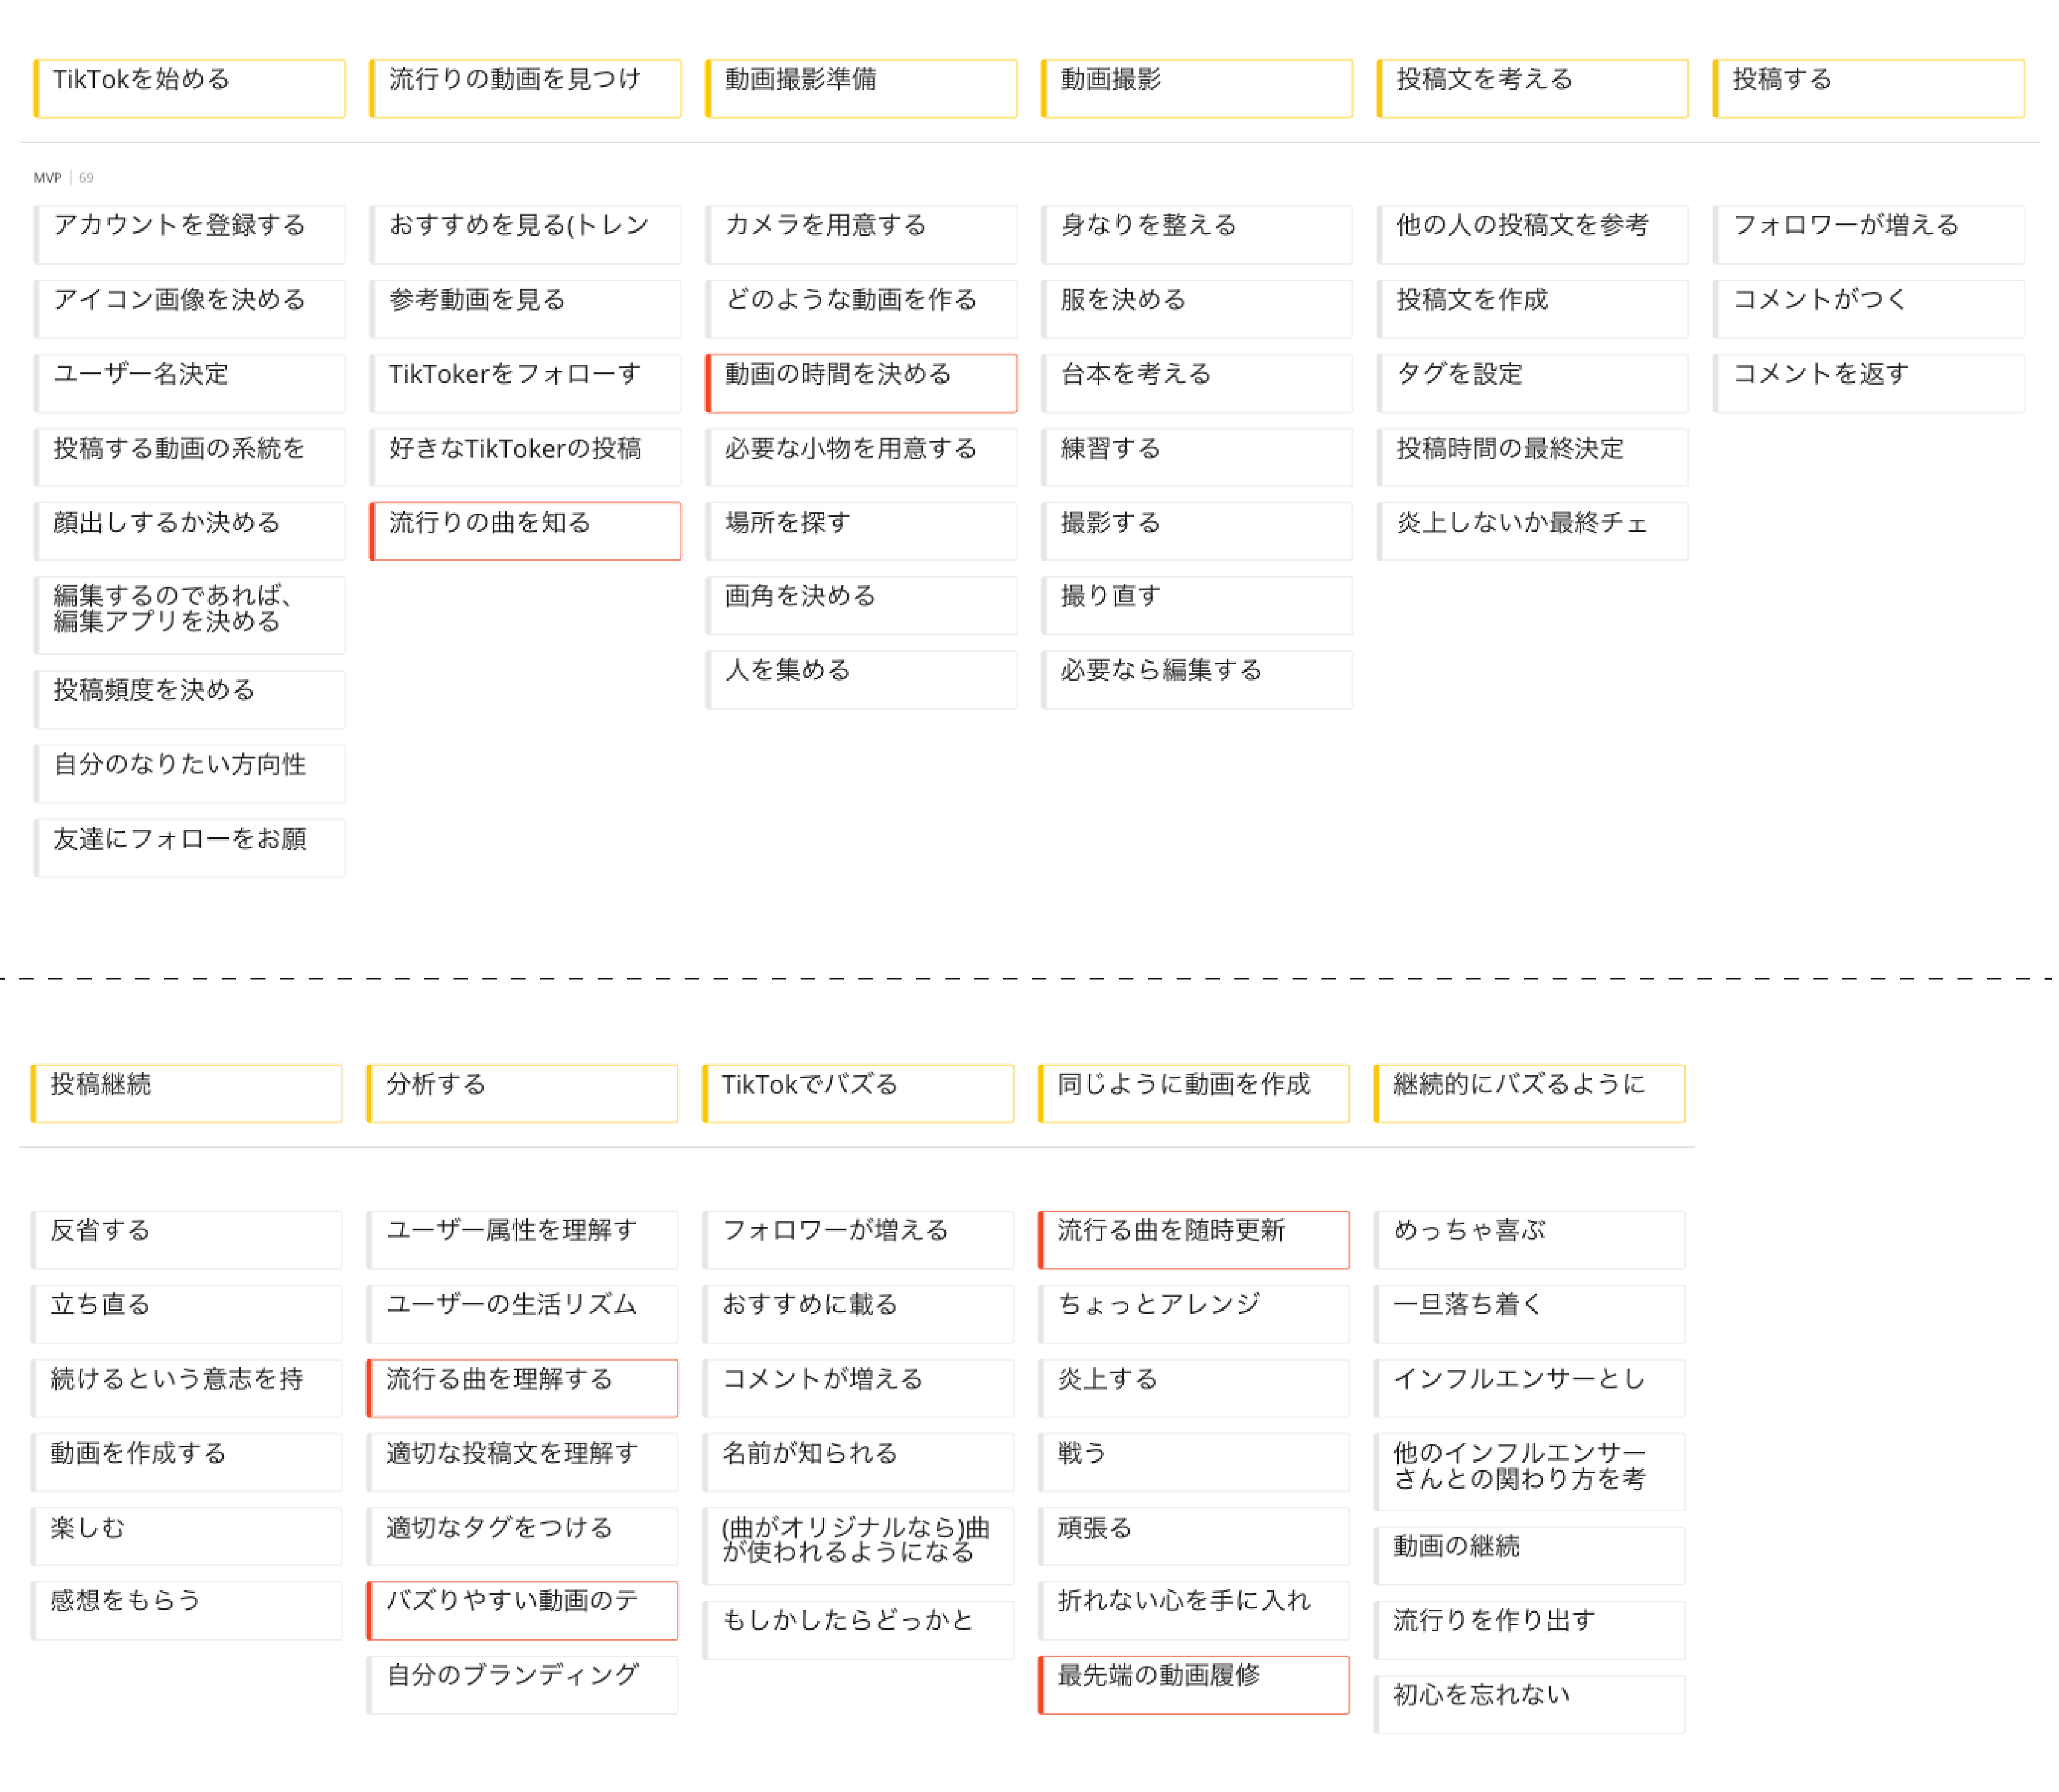
\includegraphics[width=120mm]{images/USM.png}
\label{fig:makemovie}
\caption{ユーザーストーリーマッピング}
\end{center}
\end{figure}

% しかし,他の媒体と流行しやすい楽曲が異なるため使用楽曲の選定が難しい.
研究者やマーケターがTikTokでこれから流行しそうな楽曲の見解を示してはいるものの,直感的ではないことなどが問題として挙げられる.
このようなことから,TikTokでこれから流行する楽曲や,ユーザーの使用したい楽曲が流行するかどうかを提示するシステムの開発を目標に掲げた.

TikTokで動画を投稿している人は, 流行している楽曲をTikTokのアプリケーション内にあるランキング等を利用して把握している.しかし,それらの楽曲は現在流行しているものであって, これから流行しそうな曲を把握し流行の波にいち早く乗るのには適していない.
そのため, これから流行しそうな楽曲の提示を行うことが必要である.
また, 図3.1下段の「分析する」にある「流行る曲を理解する」を達成するために特徴量の提示を行う必要もあるとも考えた.

% これを達成するには,システムがTikTokで流行する楽曲を予測できること,ユーザーが使用したい楽曲が流行しやすいかどうかを提示すること,ユーザーが直感的にシステムの操作ができることが必要だと考えた.
% また,ユーザーが流行しやすい楽曲の傾向を掴むために,楽曲の特徴を提示することも必要である.
以上から,今回我々がシステムを開発する上で求められる要件は以下の4つと考えた.
\begin{description}
\item [R1] TikTokで流行する楽曲を予測し,提示する
\item [R2] TikTokで流行する楽曲の特徴を提示する
\item [R3] ユーザーが使用したい楽曲が流行しやすいかを提示する
\item [R4] ユーザーが直感的に扱うことができる
\end{description}
これらの要件を実現するために必要な楽曲データの処理について第\ref{section:data-processing}章で,ユーザーインタフェースについて第\ref{section:user-interface}章で述べる.

\chapter{データ処理}
\label{section:data-processing}

流行する楽曲の予測および楽曲の特徴を可視化するために,Spotify APIから取得した以下の13個の音楽特徴を使用した.
\begin{description}
  \item[acousticness] トラックがアコースティック音楽かどうかを表す数値.
    \item[danceability] トラックの踊りやすさを表した数値.
    \item[energy] トラックのエネルギッシュさを表した数値.
    \item[instrumentalness] トラックにボーカルが含まれていないかどうかを表した数値.
    \item[liveness] トラックのなかに聴衆の存在がどれくらいあるのかを表した数値.
    \item[loudness] トラックの全体の音の強さ・大きさを示すデシベル数(dB).
    \item[speechiness] トラック内の話し言葉の存在を表す数値.
    \item[tempo] トラック全体で見込まれる毎分時のビート(BPM)を表す数値.
    \item[time\_signature] トラックの拍子を表す数値.
    \item[valence] トラックのポジティブ度を表す数値.
    \item[mode] トラックのキーがマイナーかメジャーかを表す数値.
    \item[key] トラックのキーを表す数値.
    \item[duration\_ms] トラックの長さをmillisecondsで表した数値.
\end{description}
さらに,楽曲の歌詞に基づいた特徴を可視化するために,Musixmatch Developer API(\url{https://developer.musixmatch.com/})から取得した歌詞を使用した.
なお,API使用枠の制限により,歌詞の冒頭部分のみを使用している.
Musixmatch Developer APIから取得された歌詞のブロックをセクションと呼ぶ.
セクションは,Aメロ,Bメロ,サビ等の楽曲構成ではなく,APIから得た歌詞の行間ごとの集合である.

\section{流行楽曲の予測}
\label{section:prediction}
BuzzLeadでは,過去にTikTokで流行した楽曲,していない楽曲を用いて任意の楽曲がTikTokで流行しやすいかどうかを判定する.
TikTokで流行した楽曲は,TikTok Chartsにランクインした楽曲のうちSpotifyがデータを提供しているものを使用した.
TikTok Chartsで週ごとに掲載される20曲のうち,Spotifyがデータを提供している楽曲は15曲程度である.
流行した楽曲と同程度の曲数の流行していない楽曲を取得するために,Spotify ChartsのWeekly Top Songs Japanに掲載される200曲のうち下位15曲を使用した.

分類アルゴリズムには,ロジスティック回帰,ランダムフォレスト,サポートベクターマシンの3つを使用した.
上記の流行した楽曲・流行していない楽曲を用いて,それぞれのアルゴリズムで二値分類モデルの学習を行った.
説明変数には,Spotify APIから取得した音楽特徴を使用した.
3つのモデルに楽曲の音楽特徴を入力し,流行した楽曲だと分類したモデルの個数を楽曲の流行度として0~3の値で提示した.

\section{歌詞特徴}

楽曲の歌詞の特徴を可視化するために,以下のポジティブ度と韻踏み度を算出した.

\begin{description}
  \item[ポジティブ度] ポジティブ度は,歌詞に出てくる単語のうち,どれくらいポジティブな単語があるかを100点満点で表したものである.
ネガティブな単語もポジティブな単語もなかった場合はポジティブ度を50としている.
    % XXX 句とは?
    セクションのポジティブ度は,行ごとにネガティブな単語・ポジティブな単語の数を数え,ポジティブな単語の百分率の平均をとったものである.
    また,全体でのポジティブ度はセクションのポジティブ度の平均をとったものである.
    単語のネガティブ・ポジティブの判定には,日本語感情分析ライブラリのoseti(\url{https://github.com/ikegami-yukino/oseti})を使用した.
  \item[韻踏み度] 韻踏み度は,歌詞の中でどのくらい韻を踏んでいるかを100点満点で表したものである.
    韻踏み度の算出には,歌詞の形態素解析によって日本語を母音のみに変換し,同じセクション内で該当行以降に出てくる歌詞の単語同士を比較する.
    ここで,母音が何文字一致しているかを取得し,1文字だけ一致の場合はスコアを0.01,2文字以上の場合は1とする.
    このとき,同じ言葉の場合は繰り返しとみなしてスコアを0とする.
    セクション,全体の韻踏み度は共にスコアの単純平均を取っている.
\end{description}



\chapter{ユーザーインターフェース}
\begin{figure*}[htb]
\begin{center}
\includegraphics[width=150mm]{images/BuzzLead_edit_last.png}
\label{fig:BuzzLead}
\caption{
  TikTokの流行曲予測システムBuzzLeadにおけるメインページのスクリーンショット.
  (a)ピックアップビュー:選択した週に流行すると予測された楽曲を一覧表示する.
  (b)特徴量比較ビュー:ピックアップビューに表示されている楽曲の音楽特徴量を平行座標プロットによって表示する.
  (c)音楽特徴量ビュー:選択された楽曲の音楽特徴量を表示する.
  (d)歌詞概要ビュー:歌詞で多く使われている単語と,そのポジティブさ・ネガティブさをワードクラウドで表示する.
  (e)歌詞特徴量ビュー:歌詞のポジティブ度と韻踏み度を表示する.
}
\end{center}
\end{figure*}

\label{section:user-interface}
% 図\ref{fig:BuzzLead}は,BuzzLeadのメインページのスクリーンショットである.
% メインページは,ピックアップビュー(図\ref{fig:BuzzLead}(a))と特徴量比較ビュー(図\ref{fig:BuzzLead}(b)),曲詳細ビューの3つのビューで構成されている.
% さらに,曲詳細ビューは,音楽特徴量ビュー(図\ref{fig:BuzzLead}(c))と歌詞概要ビュー(図\ref{fig:BuzzLead}(d)),歌詞特徴量ビュー(図\ref{fig:BuzzLead}(e))の3つのサブビューで構成されている.
図5.1は,BuzzLeadのメインページのスクリーンショットである.
メインページは,ピックアップビュー(図5.1(a))と特徴量比較ビュー(図5.1(b)),曲詳細ビューの3つのビューで構成されている.
さらに,曲詳細ビューは,音楽特徴量ビュー(図5.1(c))と歌詞概要ビュー(図5.1(d)),歌詞特徴量ビュー(図5.1(e))の3つのサブビューで構成されている.
ピックアップビューはR1を,特徴量比較ビューと曲詳細ビューはR2を達成することが狙いである.
また,R3を達成するために,ユーザーが自由に楽曲を検索し,その特徴を調べるための楽曲検索機能を提供する.

\section{ピックアップビュー}
ピックアップビューでは,週ごとに予測された流行曲のリストが表示される.
% XXX 適当に書いたけどこの理解でOK?
Spotify Chartsからprevious\_rankがNEW,RE-ENTRY,15位以上ランクアップした楽曲のうち,\ref{section:prediction}の方法で算出した流行度が1~3の楽曲をピックアップ曲とした.
週ごとに\ref{section:prediction}の手法を用いて得られたピックアップ曲を表示している.
% XXX 3段階?
また,4段階ある流行度はアイコンを用いて表している.
流行度の高い楽曲を上部に表示しているが,ユーザーはスクロールすることで流行度が比較的低い楽曲を見ることができる.
加えて,ユーザーは日付を選択することで過去のピックアップ曲を見ることができる.

\section{特徴量比較ビュー}
特徴量比較ビューでは,ピックアップビューで表示されている楽曲の音楽特徴量を比較することができる.
% XXX 重要度とは?
13個の音楽特徴のうち,重要度の高かった8項目を平行座標プロットで表している.
平行座標プロット中の折れ線は,PCではホバー,スマートフォンではタップによって選択することができ,選択された折れ線のみがフォーカスされ,対応した曲名が表示される.
折れ線の色は流行度に対応しており,水色,紫,赤の順に流行度が高くなっている.

%2.4
\section{曲詳細ビュー}

曲詳細ビューでは,選択された楽曲の特徴が3つのサブビューで表示される.

\subsection{音楽特徴量ビュー}
音楽特徴量ビューでは,Spotify API から取得した13個の音楽特徴がそれぞれどの値を取っているかを表示している.
13個の音楽特徴のうち0〜1で表せる8つの項目をレーダーチャートで表示している.
loudnessは-60〜0の値を取るため,0〜1に正規化している.
また,レーダーチャートに含まれていない項目は左側にテキストで表示している.
keyとmodeは組み合わせて調という表記で示している.

\subsection{歌詞概要ビュー}
歌詞概要ビューでは,歌詞に出現する名詞・動詞・形容詞を形態素解析によって抽出しワードクラウドで表している.
文字の大きさが単語の出現回数を表しており,文字が大きいほど出現回数が多い.
また,文字の色は,赤がポジティブ,青がネガティブ,グレーがどちらでもない単語を表している.

\subsection{歌詞特徴量ビュー}
歌詞特徴量ビューでは,ポジティブ度と韻踏み度を歌詞全体とセクションごとに分けて表示している.
グラフのノードにホバーすると点数が表示される.
また,横軸のセクションにホバーすると歌詞が表示される.
ただし,第\ref{section:data-processing}章で述べた通り,現段階では冒頭の歌詞しか取得できていないため,歌詞の全表示はできていない.

\section{楽曲検索}
ヘッダーの虫眼鏡アイコンからユーザーが自由に楽曲を検索し,その楽曲自体と,その楽曲と似た流行度の高い楽曲の詳細を調べることができる.
検索フォームから楽曲名,またはアーティスト名を入力すると,該当する楽曲が一覧表示される.そこに表示されている楽曲を選択することで,その楽曲の詳細ページ(図5.2)に遷移する.
詳細ページでは,メインページと同様の曲詳細ビュー(図5.2(c))によって選択された楽曲の特徴が表示される.
さらに,選択された楽曲の流行度を示すアイコン(図5.2(a))が表示され,その楽曲の流行度を知ることができる.
また,Spotify APIから取得した類似曲のうち,流行度が1~3の楽曲のリスト(図5.2(b))が表示される.

\begin{figure}[htb]
\begin{center}
\includegraphics[width=120mm]{images/BuzzLead_search.png}
\label{fig:search}
\caption{
  TikTokの流行曲予測システムBuzzLeadにおける楽曲詳細ページのスクリーンショット.
  (a)流行度ビュー:選択した楽曲の流行度をアイコンで表示する.
  (b)類似曲ビュー:Spotify APIから取得した類似曲のうち,流行度が1~3の楽曲のリストを表示する.
  (c)曲紹介ビュー:5.1と同様に選択された楽曲の音楽特徴量を表示する.
}
\end{center}
\end{figure}


\section{その他}
\begin{description}
  \item[マイページ] ユーザーは,閲覧した楽曲を曲名の横にあるハートボタンからマイページに登録でき,登録した楽曲はマイページから参照することができる.
    マイページはヘッダーのハートボタンから開くことができる.
    マイページでは,登録された楽曲の一覧と楽曲詳細が表示される.
  \item[試聴] BuzzLeadでは楽曲のサムネイル画像をクリックすることで,実際に楽曲を数十秒聴くことができる.
  \item[レスポンシブデザイン] TikTokユーザーはPCよりもスマートフォンを使うことが多いと考えられるため,スマートフォンにも対応したレスポンシブデザインとなっている(図5.3).スマートフォンではトップ画面にピックアップビュー(図5.3(a))と特徴量比較ビュー(図5.3(b))を表示し, 楽曲を選択すると曲詳細画面に遷移し, そこで音楽特徴量ビュー(図5.3(c)), 歌詞概要ビュー(図5.3(d)), 歌詞特徴量ビューを表示している.
  
\end{description}

\begin{figure}[htb]
\begin{center}
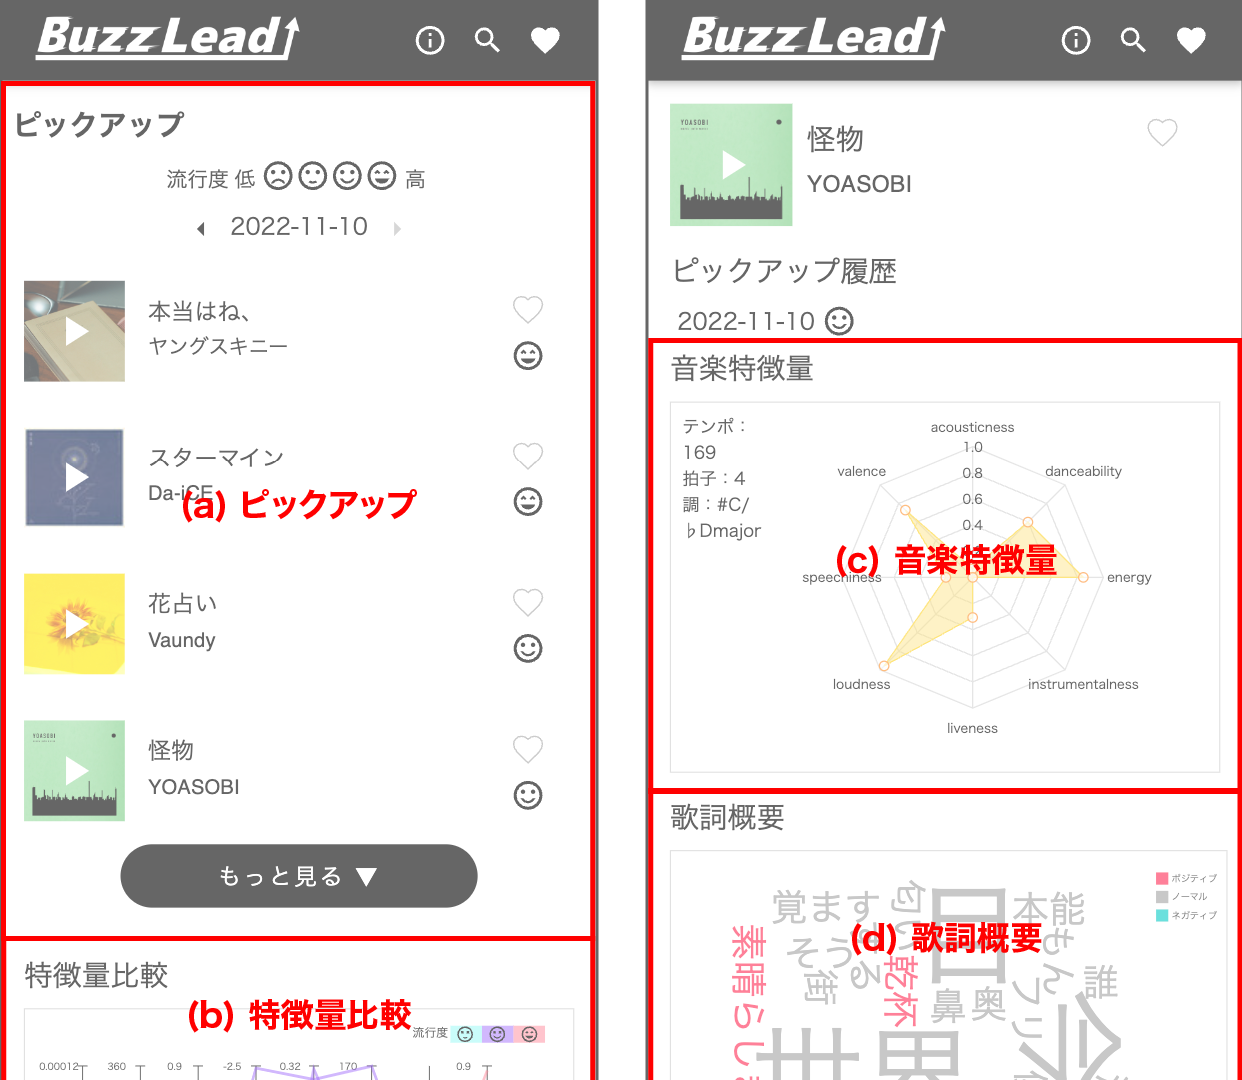
\includegraphics[width=120mm]{images/BuzzLead_sp.png}
\label{fig:smartphon}
\caption{
  TikTokの流行曲予測システムBuzzLeadのスマートフォンでのトップページと楽曲詳細ページのスクリーンショット.
  (a)ピックアップビュー:5.1と同様に選択した週に流行すると予測された楽曲を一覧表示する.
  (b)特徴量比較ビュー:5.1と同様にピックアップビューに表示されている楽曲の音楽特徴量を平行座標プロットによって表示する.
  (c)音楽特徴量ビュー:5.1と同様に選択された楽曲の音楽特徴量を表示する.
  (d)歌詞概要ビュー:5.1と同様に選択された楽曲の歌詞概要を表示する.
}
\end{center}
\end{figure}



\chapter{評価}
% R1~R4の要件を我々が開発したシステムが満たしているかは,hoge,hoge,hogeであることを確かめる必要があると考え,以下3項目を調査するために,予測の正確さの調査とユーザーテストを行った.
R1〜R4の要件を我々が開発したシステムが満たしているかどうかを確かめるために,以下の3項目の調査を行なった.
\begin{description}
\item [C1] 予測した楽曲が実際に流行したか
\item [C2] ユーザーが流行する楽曲の特徴を把握できたか
\item [C3] ユーザーが直感的にシステムを扱えたか
\end{description}


\section{予測の正確さ}
C1を明らかにするために,BuzzLeadでの流行曲の予測がどれくらい当たったかの割合を表\ref{table:predict_accuracy}に集計した.
TikTokで流行したかどうかはTikTok Chartsに楽曲名が載っているかどうかで判断している.
集計した結果の平均は12\%となった.
このような値になった原因として,まだ流行していない楽曲として集めた楽曲のデータにそもそもTikTokのランキングの曲が含まれていないことや,そもそもTikTok特有の楽曲などのSpotify Chartsにはない楽曲は取得できないことが考えられる.
前者に対しては,まだ流行していない楽曲として集める楽曲の幅を増やすことで解決できると考えている.
予測した楽曲が一切含まれていない週もいくつかあるが,9/29のように流行する楽曲を3割当てている週もある.
8/4の1曲,9/1の3曲,9/15の1曲,10/6の1曲,10/20の1曲はこれまでランキングに載っておらず,その週から流行し始めた楽曲をあらかじめ予測できていた.
%ユーザーに次流行する楽曲を提示するという目標を達成できたのではないだろうか.
また,これ以外の楽曲も,前の週に流行していた楽曲が次週も流行するのかどうかという点で,使用音源の流行を気にするユーザーが楽曲を選ぶ指標になると考えられる.
% だが,予測が当たる割合は低いので高めていきたい.
これらから,改善の余地はあるもののR1を満たすことができたと考えた.
\begin{table}[hbt]
% \begin{table*}[hbtp]
  \caption{予測の正確さ}
  \label{table:predict_accuracy}
  \centering
  % \begin{tabular}{ll}
  \begin{tabular}{c c c}
    \hline
    日付  & 割合  & 割合(\%)\\
    \hline \hline
    7/7 & 2/10 & 20\\
    7/14 & 2/12 & 17\\
    7/21 & 1/13 & 8\\
    7/28 & 0/9 & 0\\
    8/4 & 1/7 & 14\\
    8/11 & 0/9 & 0\\
    8/18 & 0/9 & 0 \\
    8/25 & 1/12 & 8\\
    9/1 & 3/15 & 20\\
    9/8 & 1/10 & 10\\
    9/15 & 2/9 & 22\\
    9/22 & 3/16 & 19\\
    9/29 & 2/6 & 33 \\
    10/6 & 1/11 & 9\\
    10/13 & 0/9 & 0\\
    10/20 & 1/11 & 9\\
    10/27 & 1/8 & 13\\
    % 11/3 & 1/4\\
    % 11/10 & /11\\
    \hline
  \end{tabular}
\end{table}

% \begin{table}[hbt]
% % \begin{table*}[hbtp]
%   \caption{予測の正確さ}
%   \label{table:predict_accuracy}
%   \centering
%   % \begin{tabular}{ll}
%   \begin{tabular}{c c c}
%     \hline
%     日付  & 割合  & 割合(\%)\\
%     \hline \hline
%     7/7 & 2/10 & 20\\
%     7/14 & 2/12 & 17\\
%     7/21 & 1/13 & 8\\
%     7/28 & 0/9 & 0\\
%     8/4 & 1/7 & 14\\
%     8/11 & 0/9 & 0\\
%     8/18 & 0/9 & 0 \\
%     8/25 & 1/12 & 8\\
%     9/1 & 3/15 & 20\\
%     9/8 & 1/10 & 10\\
%     9/15 & 2/9 & 22\\
%     9/22 & 3/16 & 19\\
%     9/29 & 2/6 & 33 \\
%     10/6 & 1/11 & 9\\
%     10/13 & 0/9 & 0\\
%     10/20 & 1/11 & 9\\
%     10/27 & 1/8 & 13\\
%     11/3 & 1/4 & 25\\
%     11/10 & 1/11 & 9\\
%     11/17 & 1/9 & 11 \\
%     11/24 & 1/14 & 7 \\
%     12/1 & 2/6 & 33 \\
%     12/8 & 0/13 & 0 \\
%     12/15 & 2/8 & 25 \\
%     12/22 & 3/11 & 27\\
%     12/29 & 2/11 &  18\\
%     1/5 & 0/25 & 0 \\ 
%     1/12 & 2/15 & 13\\
%     1/19 & 1/13 & 8\\
%     \hline
%   \end{tabular}
% \end{table}
    
\section{ユーザーテスト}
C2,C3を明らかにするためにユーザーテストを行った.
ユーザーテストに参加した実験参加者に,実際にBuzzLeadを操作してもらい,その後アンケートに回答してもらった.
% 最終的に33名の回答が得られた.
% ダンスや配信,音楽に関わっている団体にSNSで拡散をした.実際にBuzzLeadを使用してもらい,アンケートを行った結果,33名の回答が得られた.
\subsection{実験参加者}
実験参加者は,情報科学を専攻する大学生13名と,ダンスや配信,音楽に関わっている団体への募集で集まった20名の33名である.
33名のうち,TikTokを普段利用する人は13名,その中でも配信をする人は3名だった.
また,TikTok以外のツールで動画の配信を行っている人は6名だった.
%88\%が20~25歳,その他は10代と25~29歳だった.また,

\subsection{アンケート結果}
BuzzLeadで表示しているピックアップ曲や,楽曲詳細などのビューについての評価をするために,5段階評価(5:そう思う,4:ややそう思う,3:どちらともいえない,2:あまりそう思わない,1:全くそう思わない)で次のQ1〜Q5の質問を行った.
\begin{description}
\item [Q1] 選択した楽曲の音楽の特徴を知ることができた
\item [Q2] 選択した楽曲の歌詞の特徴を知ることができた
\item [Q3] 選択した楽曲の歌詞がどれくらいポジティブかを知ることができた
\item [Q4] 選択した楽曲の歌詞がどれくらい韻を踏んでいるかを知ることができた
\item [Q5] 自分の検索した楽曲の流行度を知ることができた
\end{description}
Q1〜Q5の結果(図2)から多くの実験参加者が楽曲詳細のビューを用いて音楽,歌詞両方の特徴を掴むことができていることがわかる.
これより,R2,3を満たしていると考えられる.
% 一方Q6では票がバラけており,お気に入りに登録した曲の共通点を見つけることが少し難しかったと考えられる.
% これは,ピックアップの下にある特徴量比較のようなビューをマイページに設けていなかったことが原因と考えられるため,そのような複数曲を比較できるビューをマイページにも設けるようにしていきたい.

システムの操作が関わるQ1〜Q5に加え,楽曲検索を行えたかどうか,マイページにお気に入りを登録することができたかどうかといった質問では,30名以上が4か5を選択しており,実験参加者が直感的にシステムを扱うことができていたと考えられる.

一方,実験参加者に対して「ピックアップ」に表示されているのはどのような楽曲か聞いたところ,今,TikTokで流行っている楽曲と回答した人が42\%,正解であるこれからTikTokで流行しそうな楽曲と回答した人が27\%,その他が31\%とこちらの意図が伝わっていない結果となった.
この結果から,このアプリケーションの目的が実験参加者にしっかり伝わっていなかったことと,流行度という言葉を既に流行しているものを表していると認知した実験参加者が一定数いたためだと考えられる.
流行度やピックアップという題名を考え直すと共にUIの改善を行っていきたい.

以上のことから,一部UIに改善点はあるもののR4を達成することができたと考える.
\begin{figure}[htb]
\begin{center}
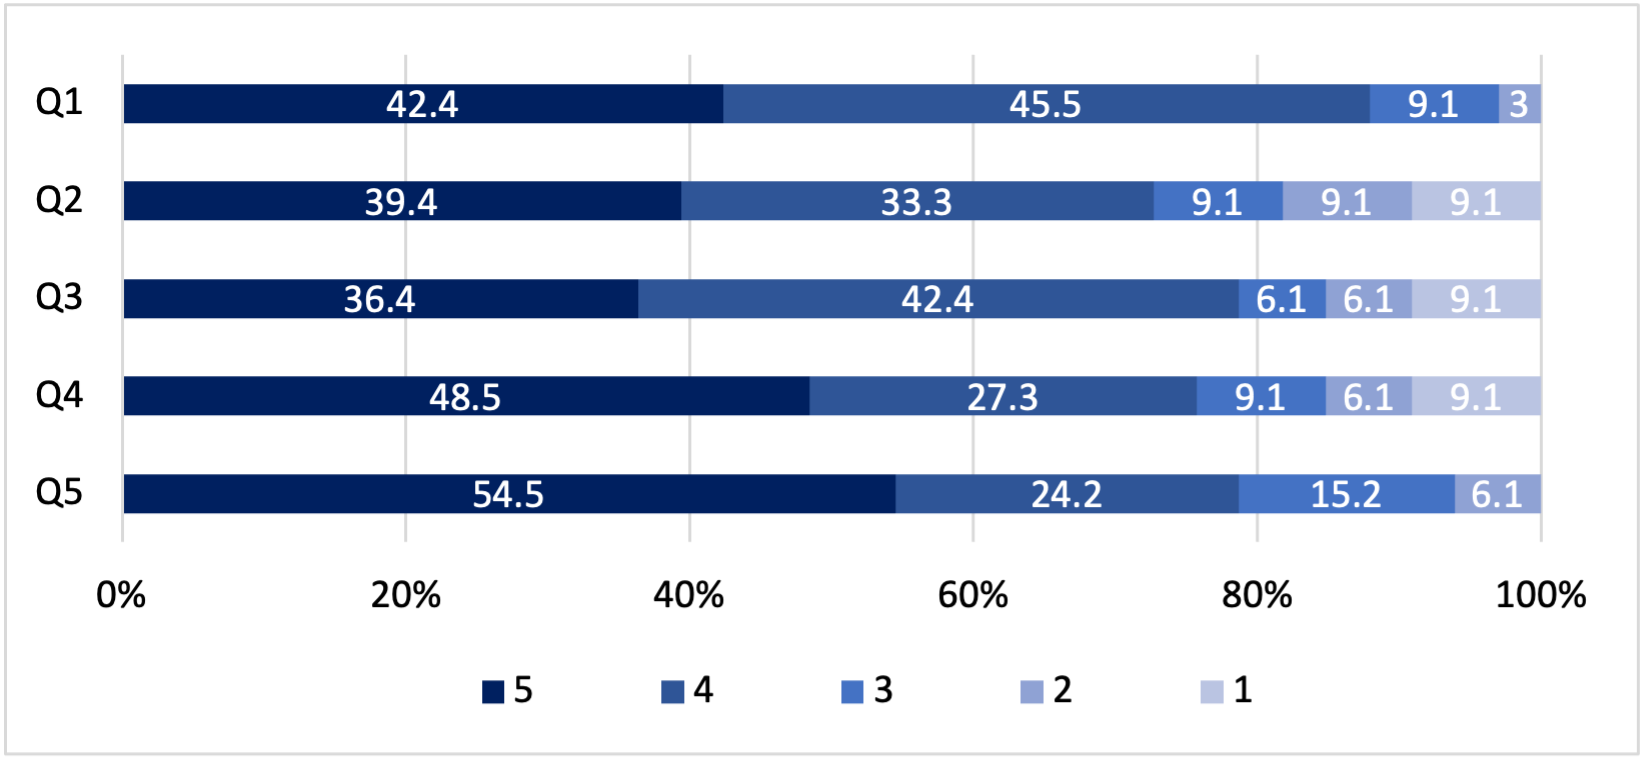
\includegraphics[width=80mm]{images/feature.png}
\label{table:detail}
\caption{楽曲詳細}
\end{center}
\end{figure}

%前向きな意見
%古い曲を調べると流行度が低いことが多かったので,ある意味正確なように感じました.ただ,今実際にtiktokで流行しているものを知らないので本当に流行するのかどうかはわからないと思いました.
%可視化についても流行度を色で,音楽の特徴量を折れ線で表現することで1つのチャートで表せていたりしていて直感的に理解できるように感じました.
%流行っていた曲の特徴を知ることができたので,これから流行する曲がどのような曲調のものなのかを少し予想できるようになりました.

%改善点
%ピックアップ履歴というところに流行度の推移が表示されており,これが何かわからなかった.
%音楽に対して詳しくないので音楽の特徴を見ても,何が理由で流行しそうなのかわからなかった.
%自分が見たのが悪かったのがdanceability,energy,loudnessが大体同じくらい高いしspeechiness,instrumentalnessは大体0で差を感じなかった.
%歌詞のポジティブとネガティブ,曲の韻踏み度とポジティブ度,それらが流行しそう度とどう関係があるのかわからない←未実装の伝達不足
%曲同士の比較がもっとできると嬉しい
%月や年単位でのピックアップorランキングの表示
%その他UIの改善


%\subsection{サービス全体について}
最後にサービス全体についても5段階評価でQ6〜Q8の質問を行った.
\begin{description}
\item [Q6] 流行しそうな楽曲を知ることができた
\item [Q7] 流行しそうな楽曲の特徴を掴むことができた
\item [Q8] 実際におすすめされた楽曲を使って動画を投稿してみようと思った
% \item [Q10] オススメされた流行度の高い楽曲が実際に流行しそうだと思った
\end{description}
その結果を図3に表す.
Q6,Q7に関しては前向きな評価を多く得ることができ,R1,R2を達成できたと考えることができる.
% また,Q10でも多くの人が5か4を回答していることから提示した曲が直感的にも流行しそう
一方,Q8では5,4をつけた人が少なかった.
今回の実験参加者に,TikTokで動画投稿をしている人が3名しかいないからだと考えられる.
TikTok投稿を行なっている人の評価は4,3,1であった.
% これは5.2.1にもあるように,今回の参加者に,そもそもTikTokで動画投稿をしている人が少ないからだと考えたが実際はそうでもなかった.Q9で4,5の評価をしてくれた人は,動画投稿をする人が2名,しない人が3名だった. また,実際にTikTok投稿を行なっている人の評価は4,3,1であった.

\begin{figure}[htb]
\begin{center}
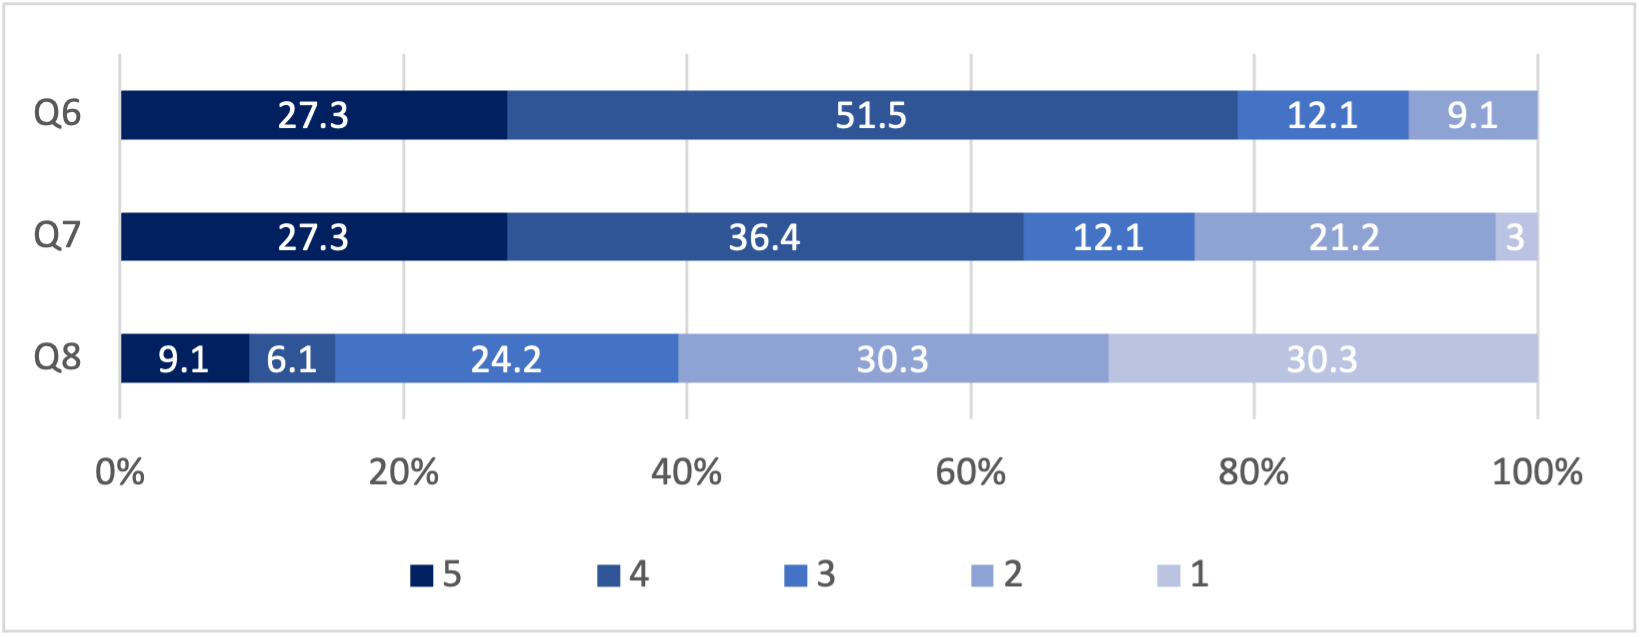
\includegraphics[width=80mm]{images/all.png}
\label{table:total}
\caption{サービス全体について}
\end{center}
\end{figure}

以下は,実験参加者の自由記述によるコメントの抜粋である.
\begin{itemize}
\item 古い曲を調べると流行度が低いことが多かったので,ある意味正確なように感じました
\item 流行っていた曲の特徴を知ることができたので,これから流行する曲がどのような曲調のものなのかを少し予想できるようになりました.
\item 歌詞のポジティブとネガティブ,曲の韻踏み度とポジティブ度,それらが流行しそう度とどう関係があるのかわからない
\item 月や年単位でのピックアップorランキングの表示
\end{itemize}
コメントから,実験参加者は流行度に納得していることや流行する楽曲の特徴を掴めていることがわかる.
一方で,歌詞特徴量が流行度とどう関係しているかわからないという意見もあった.
これは,流行度の算出に歌詞特徴量を使用していないことや,特徴量比較ビューに歌詞特徴量を表示していないためだと考えられる. 
現時点で,歌詞取得が楽曲の冒頭部分しかできていないため音楽特徴量のみを使用しているが,全歌詞を使用した歌詞特徴量の採用は今後の課題である.
最後に,月や年単位でのピックアップあるいはランキングの表示をしてもらいたいとの意見もあったので検討していきたい.


\chapter{考察}
本研究ではTikTokでこれから流行する楽曲や,ユーザーの使用したい楽曲が流行するかどうかを提示するシステムの開発を目標に掲げ,4つのシステム要件を定めた.

R1に関しては,6.1にもあるように一部予測はできているが精度が低い結果となった.
しかし, TikTok Chartsの順位が大きく入れ替わる際に予測した楽曲がランクインしていることもあり,精度は低いながらも要点はつかめている印象を受けた.
今回はこのような精度となったが,歌詞を利用した分類や,楽曲全体ではなくサビやAメロといった楽曲の一部分を対象にした分類を行うと,よりTikTokの傾向に沿った予測ができるのではないかと考えている.

R2に関しては,6.2.2にあるように多くのユーザーが楽曲の特徴を把握できていた.
しかし歌詞が冒頭しか取得できていないことから,楽曲全体の歌詞の特徴を掴むのには適していない状態となってしまった. 
歌詞の取得先を変更するなどの改善を行っていきたい.

R3に関しては,ユーザーが検索した楽曲の流行度をアイコンで提示することで達成できた.
また,流行度の高い類似曲を提示することでユーザーの嗜好に合致し,かつ流行しやすい曲を把握することが可能になった.

R4に関しては,タイトルの付け方によってユーザーの誤解を招いてしまう部分があったが,多くのユーザーが問題なくアプリケーションを操作していた. 
また,スマートフォンを利用してユーザーアンケートに回答したユーザーは45\%を占めていた.この結果から,レスポンシブデザインを取り入れたことにより,TikTokを使用しているユーザーのアンケート協力の件数を増やすことができたと感じている.

全体を通して,予測の精度は改善の余地があるがアプリケーションとしては要件を満たすものが作成できた.
TikTokで自身のコンテンツを流行させたい人はもちろんだが,著者の一人も一時期TikTokの投稿をする際に使用楽曲を選ぶ煩わしさを感じていたので,そういった人達の助けにもなることを願っている.

% 実際やる前から曲の共通点出すの難しくね?ってなってて、わかったらやばいねって話を音楽友達としてたり。で、実際学習させてみてもまぁそうよねって感じではあったので、そうだよなって感じではある。世の中ほんと色んな楽曲があって、これが一番流行る!とかは一概に言えないんだなって再認知したというかなんというか。
% そんな中でも、大バズりしてる楽曲は流行度が高いことが多くて、なんらかはあるんだろうなと思ったり、でもぱっと見わからない。誤差なんか。
% TikTok一回バズるとだいたいその曲が数週間ずっとランキング上位にいるんだけど、それがひっくり返るタイミングで予想曲当ててたのはちょっと胸熱だった。
% 歌詞を利用しての分類や, 楽曲全体ではなくサビやAメロといった一部分のみでの分類等を行うとまた違った結果になるのではないかと思っている。TikTokは15秒とかしか使わないから、そこだけで見てみたいっていうやつ。
% ユーザーインターフェースというかアプリケーションとしての機能はそれなりにできていたと思う。レスポンシブデザインも用意して、実際にテストでスマートフォンを使うユーザーもいて狙い通りだった。一部文言での伝達ミス?があったりレイアウトや、楽曲再生などまだ改善点はあるけどそれっぽいものはできたのでは。
% TikTok投稿は2年前とかに一時期広報で使ってて曲選ぶのはめんどかったから、そういう人の助けになったらいいなと思ったり

\chapter{おわりに}
本研究では,TikTokで流行っている楽曲のデータを用い,楽曲選定の支援を目的としたシステムであるBuzzLeadを開発した.
音楽特徴量を用いてどのような特徴を持つ楽曲が流行するのか,自身の選んだ楽曲は流行しそうなのかを予測・提示することができた.
評価実験によって,ピックアップとしてシステムが提示した楽曲が実際に次の週のTikTok Chartsに掲載されていることが確認できた.
以上から我々の目的を達成できるシステムを開発することができたと考えられる.

一方で,改善点として挙げられるのがユーザーに目的を伝えきることができなかった「ピックアップ」という項目である.
TikTokで流行った楽曲の情報をもとに今後流行するであろう楽曲を提示するのが目的であったが,今現在TikTokで流行っている楽曲であると認識しているユーザーが42\%を占めた. 
回答の中にはSpotifyに関する項目であるというものも散見され,ここで目的が伝わりきらなかった理由について「このアプリケーションがどのようなものか理解せずにユーザーが利用している」ということが原因として考えられる.
どのような目的を持って作られたアプリケーションであるのかという文言をウォークスルーに盛り込むなどして改善を行っていきたい. 

\chapter*{謝辞}
% 先生ありがとうーーーーー
本研究を遂行するにあたり,指導教官である日本大学文理学部情報科学科尾上准教授には終始多大なご指導をいただきました.心から感謝いたします.
また,本研究の遂行にあたり,快く実験に参加頂いた皆様に感謝いたします.
% さんまのっけて大丈夫?
最後に,本研究を半年間協力して頂いた伊藤和斗氏,松永大氏をはじめ,尾上研究室の皆様には,本研究の遂行にあたり多大なご助言,ご協力を頂きました.本当にありがとうございました.

\begin{thebibliography}{10}
% \bibitem{paper0}
% 池上 真平,佐藤 典子,羽藤 律,生駒 忍,宮澤 史穂,小西 潤子,星野 悦子:
% 日本人における音楽聴取の心理的機能と個人差,
% 心理学研究,VOL.92,No.4,p.237-247(2021).

\bibitem{paper1}
矢倉 大夢,中野 倫靖,後藤 真孝: 
作業用BGMに特化した楽曲推薦システム,
情報処理学会研究報告,Vol.2016-MUS-112,No.3(2016).

\bibitem{paper2}
佐久間廉,伊藤 克亘: 
投稿データを利用した動画投稿者のためのBGM推薦システム,
第84回全国大会講演論文集,VOL.2022,NO.1,p257-258.

\bibitem{paper10}
小野佑大,石先広海,帆足啓一郎,小野智弘,甲藤二郎:
音楽のムード分類結果を利用したホームビデオへのBGM付与支援システム,
情報科学技術フォーラム講演論文集,VOL.9,No.2,p295-296(2010年)

\bibitem{paper4}
韓語佳,中野美由紀,小口正人:
利用者の印象に基づく高齢者向け音楽推薦システム「元気フクロウ」-嗜好に合わせた適応的推薦手法の提案-,
第84回全国大会講演論文集,VOL.2022,NO.1,p535-536.

\bibitem{p\documentclass[titlepage]{jsreport}
\usepackage[utf8]{inputenc}
\usepackage[dvipdfmx]{graphicx}
\usepackage{amsmath}
\usepackage[subrefformat=parens]{subcaption}
\usepackage[T1]{fontenc}
\usepackage{url}
\usepackage{amsfonts}
\usepackage{amssymb}

\title{BuzzLead:TikTokの流行曲予測システム}
\author{日本大学情報科学科 尾上研究室4年\\5419013 渡邉みさと \\5419015 沼部恵 \\ 5419028 阿部沙亜弥}
\date{\today}

\begin{document}

\maketitle

\begin{abstract}
TikTokは動画に特化したSNSである.そのTikTokでマーケティングが増えている中で,TikTokを有効活用し自身の価値をPRしたいと考える人々が増えている.
しかし,その際にどの楽曲を使えば再生数が伸びるのかが分からず,使用楽曲の選定がTikTok参入への障害になっていることも多い.
そこでTikTokで過去に流行した楽曲のデータから次に流行しそうな楽曲を予測・提示するシステムがあればこの問題を解決できると我々は考えた.
TikTokで流行しそうな楽曲の見解については音楽関係の研究者やマーケターが示しているが,使用者がより直感的にそれらの楽曲を発見できることが必要である.
本研究では過去のデータの分析を自動的に行い,毎週流行しそうな楽曲を更新し提示できるシステム BuzzLead(\url{https://buzzlead.vdslab.jp/})を開発した.
評価実験では「システムが提示した楽曲が実際に流行しそうだ」と判断する実験参加者が大多数を占めるなど予測が有用であったと判断できた.
\end{abstract}

\chapter{はじめに}\label{chp:intro}
近年企業がマーケティング戦略としてSNSを利用することが増えている.
その波に乗じて,自身のSNSアカウントを用いてフォロワー数を伸ばし,企業に何らかのアピールをしたいと考える人や,自身の楽曲制作活動や創作ダンス,演奏などをSNSにアップすることでアーティストとしての地位を確立したいと考える人が増えてきている.
実際にSNSでの影響力の大きさからテレビ番組に起用されたり,音楽レーベルにスカウトされたり,というインフルエンサーも今では少なくない.
特に最近注目されているのがショート動画に特化したSNSのTikTok(\url{https://www.tiktok.com/})である.
テレビで特集が組まれたり,Billboard Japan(\url{https://www.billboard-japan.com/})に専門のランキングが登場したりとTikTokが注目を浴びている.

このTikTokではフォロワーが少ない状態からでもコンテンツ次第で多くのユーザーに動画が表示され,バイラル・マーケティングを行うことができるアルゴリズムが使用されている.
つまり,他のSNSに比べて新規参入者でも非常に簡単にコンテンツを流行させやすいサービスであると言える.
しかし,TikTokを利用してコンテンツを流行らせようという人々がマーケティングを始める際に参入障壁になり得るのが楽曲の選定である.
TikTokでは知名度のない楽曲でも流行しやすい一方,流行しやすい楽曲の傾向がある.
実際,音楽関係の研究者やマーケターがTikTokで流行しそうな楽曲についての見解を示している.
もし自身の創作活動に関するアピールを行うという目的があるのであれば,この波に乗れないだけでどれほど良いコンテンツでも他の大量のコンテンツに埋もれてしまう可能性がある.そしてこれは,TikTok参入の非常に大きな障壁になりうる.

TikTokは他に例を見ない短尺動画に特化したSNSであるため,他の媒体と流行しやすい楽曲が異なっている.
そのため,楽曲選定システムに関する研究は多方面で行われているが,TikTokでの流行を考慮した楽曲選定システムが必要であると考えられる.
そこで,我々はTikTokで過去に流行した楽曲のデータから次に流行しそうな楽曲を予測・提示するシステムBuzzLeadを開発した.
BuzzLeadでは,Billboard JapanのTikTok Weekly Top 20(\url{https://www.billboard-japan.com/charts/detail?a=tiktok})(以下,TikTok Chartsと呼ぶ)に掲載されている楽曲とSpotify Charts(\url{https://charts.spotify.com/charts/view/regional-jp-weekly/latest})の楽曲を使用し,流行するか否かの分類器を作成し,それを用いて流行予測を行う.


\chapter{関連研究}
本研究ではSpotifyが公開しているSpotify API(\url{https://developer.spotify.com/documentation/web-api})を使用し,音楽特徴量の分析を行う.
これらは,利用者の印象に基づく高齢者向け音楽推薦システム\cite{paper4},色彩特徴に起因する印象に合致した楽曲推薦\cite{paper5},楽曲探索を支援するための類似楽曲提示手法\cite{paper9}といった楽曲の推薦や提示をする際に解析データとして使用されている.

矢倉らの研究では作業用BGMに特化した楽曲推薦システム\cite{paper1}が,佐久間らの研究では投稿内容に応じたBGM推薦システム\cite{paper2}が,小野らの研究では音楽のムード分類結果を利用したホームビデオへのBGM付与支援システム\cite{paper10}が提案されている.
しかしいずれもTikTokに特化した楽曲推薦システムではない. 本研究では,楽曲推薦システムの中でもTikTokでの流行に焦点を当てたものを開発する. 

% 歌詞特徴量
神野らの歌詞や曲調の印象に応じた舞台照明の自動調光・調色システムの実現\cite{paper6}では,楽曲を印象付ける特徴の一つとして一小節ごとにネガティブ・ポジティブさを求めている.本研究では一小節単位ではなく,歌詞のまとまりや全体での楽曲の印象を捉えたいため,セクションと全体でネガティブ・ポジティブさを求めポジティブ度としている.
セクションの定義については後述する.
また,鍵田らの表現特徴に着目した歌詞の印象的フレーズ抽出\cite{paper3}では押韻が楽曲を特徴づけると主張されており,CAOらの研究では押韻率\cite{paper7}を求めている.
しかしここでの押韻率は歌詞の行に対して計算されており,同じ行内で韻を踏んでいた場合に対処できていない.
よって本研究では,行に対して分かち書きを行った上で押韻率を求める.



\chapter{システム要件}
「はじめに」で述べたように,TikTokでは流行しやすい楽曲を使用することが再生回数を伸ばす上で重要になってくる.
だが,既に長期間流行している楽曲を使用すると, その楽曲を使用している動画が多いためコンテンツに埋もれてしまうことがある.そのため,いかに流行の波に早く乗るかが重要となる.

図3.1は実際にTikTokに動画を投稿している人にヒアリングをしながら作成したユーザーストーリーマッピングである.
図3.1上段の「流行りの動画を見つける」にて流行の楽曲も同時に探しているが, 他の媒体と流行しやすい楽曲が異なるため使用楽曲の選定が難しい.

\begin{figure}[htb]
\begin{center}
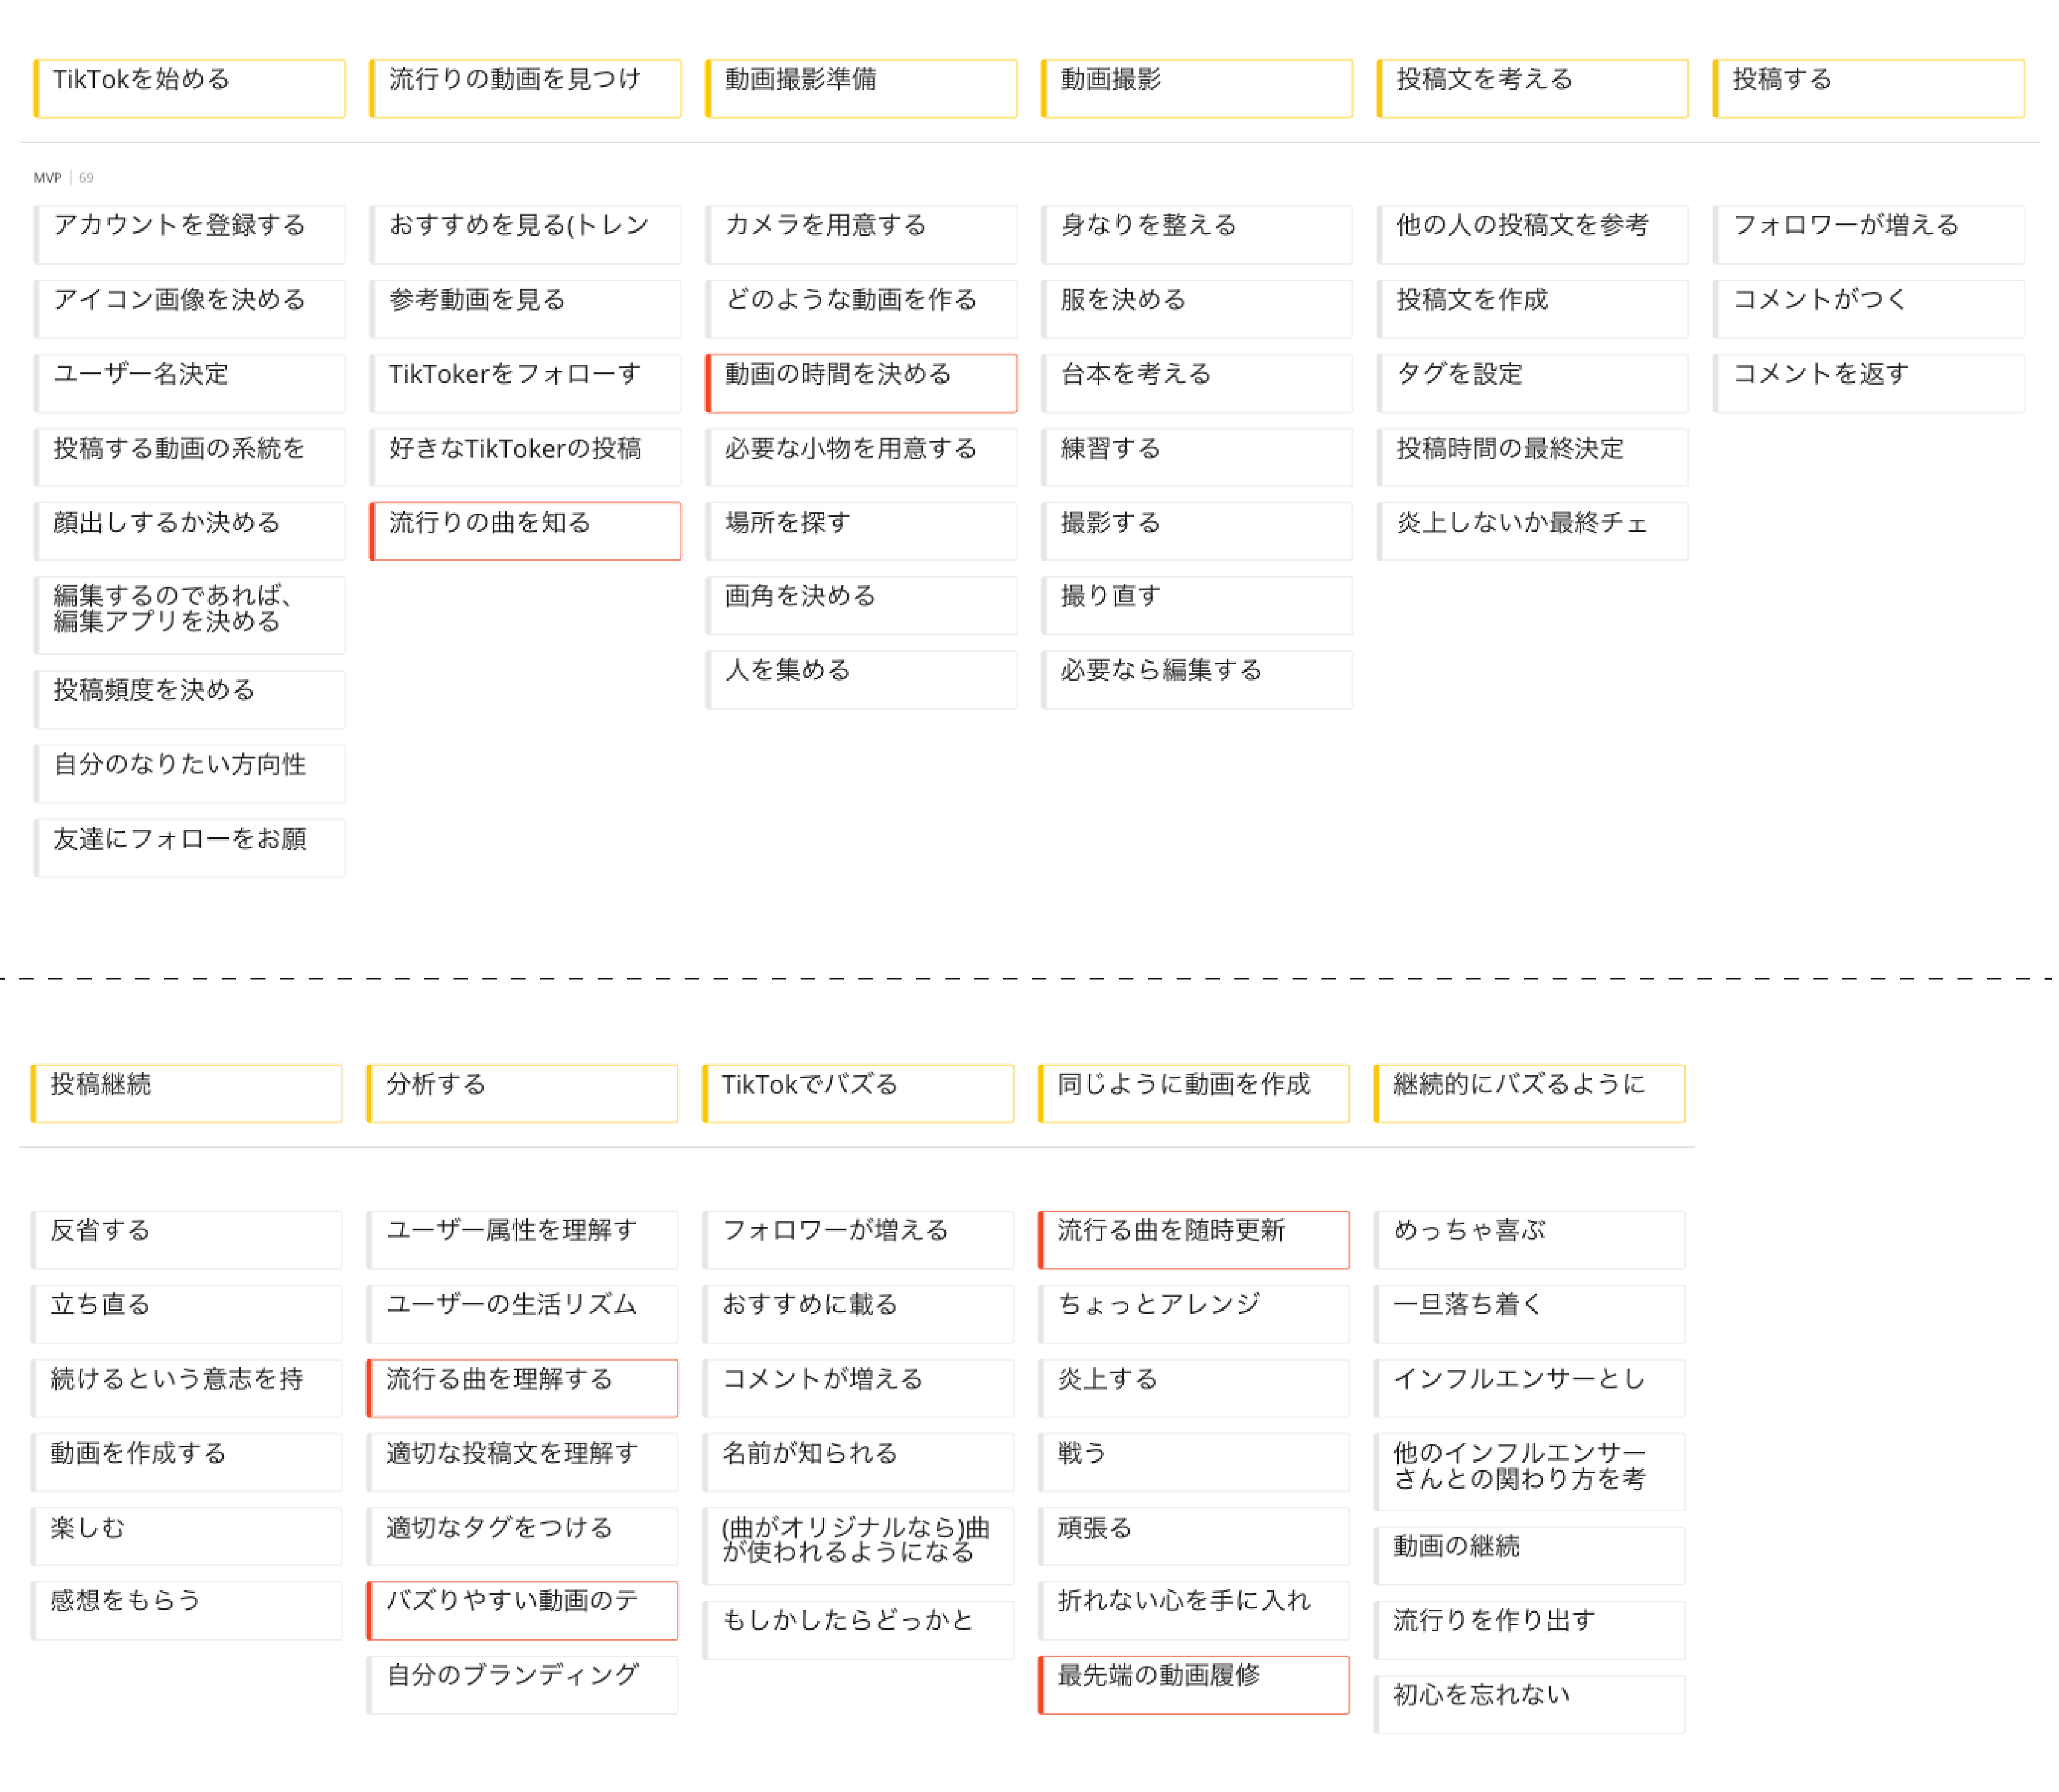
\includegraphics[width=120mm]{images/USM.png}
\label{fig:makemovie}
\caption{ユーザーストーリーマッピング}
\end{center}
\end{figure}

% しかし,他の媒体と流行しやすい楽曲が異なるため使用楽曲の選定が難しい.
研究者やマーケターがTikTokでこれから流行しそうな楽曲の見解を示してはいるものの,直感的ではないことなどが問題として挙げられる.
このようなことから,TikTokでこれから流行する楽曲や,ユーザーの使用したい楽曲が流行するかどうかを提示するシステムの開発を目標に掲げた.

TikTokで動画を投稿している人は, 流行している楽曲をTikTokのアプリケーション内にあるランキング等を利用して把握している.しかし,それらの楽曲は現在流行しているものであって, これから流行しそうな曲を把握し流行の波にいち早く乗るのには適していない.
そのため, これから流行しそうな楽曲の提示を行うことが必要である.
また, 図3.1下段の「分析する」にある「流行る曲を理解する」を達成するために特徴量の提示を行う必要もあるとも考えた.

% これを達成するには,システムがTikTokで流行する楽曲を予測できること,ユーザーが使用したい楽曲が流行しやすいかどうかを提示すること,ユーザーが直感的にシステムの操作ができることが必要だと考えた.
% また,ユーザーが流行しやすい楽曲の傾向を掴むために,楽曲の特徴を提示することも必要である.
以上から,今回我々がシステムを開発する上で求められる要件は以下の4つと考えた.
\begin{description}
\item [R1] TikTokで流行する楽曲を予測し,提示する
\item [R2] TikTokで流行する楽曲の特徴を提示する
\item [R3] ユーザーが使用したい楽曲が流行しやすいかを提示する
\item [R4] ユーザーが直感的に扱うことができる
\end{description}
これらの要件を実現するために必要な楽曲データの処理について第\ref{section:data-processing}章で,ユーザーインタフェースについて第\ref{section:user-interface}章で述べる.

\chapter{データ処理}
\label{section:data-processing}

流行する楽曲の予測および楽曲の特徴を可視化するために,Spotify APIから取得した以下の13個の音楽特徴を使用した.
\begin{description}
  \item[acousticness] トラックがアコースティック音楽かどうかを表す数値.
    \item[danceability] トラックの踊りやすさを表した数値.
    \item[energy] トラックのエネルギッシュさを表した数値.
    \item[instrumentalness] トラックにボーカルが含まれていないかどうかを表した数値.
    \item[liveness] トラックのなかに聴衆の存在がどれくらいあるのかを表した数値.
    \item[loudness] トラックの全体の音の強さ・大きさを示すデシベル数(dB).
    \item[speechiness] トラック内の話し言葉の存在を表す数値.
    \item[tempo] トラック全体で見込まれる毎分時のビート(BPM)を表す数値.
    \item[time\_signature] トラックの拍子を表す数値.
    \item[valence] トラックのポジティブ度を表す数値.
    \item[mode] トラックのキーがマイナーかメジャーかを表す数値.
    \item[key] トラックのキーを表す数値.
    \item[duration\_ms] トラックの長さをmillisecondsで表した数値.
\end{description}
さらに,楽曲の歌詞に基づいた特徴を可視化するために,Musixmatch Developer API(\url{https://developer.musixmatch.com/})から取得した歌詞を使用した.
なお,API使用枠の制限により,歌詞の冒頭部分のみを使用している.
Musixmatch Developer APIから取得された歌詞のブロックをセクションと呼ぶ.
セクションは,Aメロ,Bメロ,サビ等の楽曲構成ではなく,APIから得た歌詞の行間ごとの集合である.

\section{流行楽曲の予測}
\label{section:prediction}
BuzzLeadでは,過去にTikTokで流行した楽曲,していない楽曲を用いて任意の楽曲がTikTokで流行しやすいかどうかを判定する.
TikTokで流行した楽曲は,TikTok Chartsにランクインした楽曲のうちSpotifyがデータを提供しているものを使用した.
TikTok Chartsで週ごとに掲載される20曲のうち,Spotifyがデータを提供している楽曲は15曲程度である.
流行した楽曲と同程度の曲数の流行していない楽曲を取得するために,Spotify ChartsのWeekly Top Songs Japanに掲載される200曲のうち下位15曲を使用した.

分類アルゴリズムには,ロジスティック回帰,ランダムフォレスト,サポートベクターマシンの3つを使用した.
上記の流行した楽曲・流行していない楽曲を用いて,それぞれのアルゴリズムで二値分類モデルの学習を行った.
説明変数には,Spotify APIから取得した音楽特徴を使用した.
3つのモデルに楽曲の音楽特徴を入力し,流行した楽曲だと分類したモデルの個数を楽曲の流行度として0~3の値で提示した.

\section{歌詞特徴}

楽曲の歌詞の特徴を可視化するために,以下のポジティブ度と韻踏み度を算出した.

\begin{description}
  \item[ポジティブ度] ポジティブ度は,歌詞に出てくる単語のうち,どれくらいポジティブな単語があるかを100点満点で表したものである.
ネガティブな単語もポジティブな単語もなかった場合はポジティブ度を50としている.
    % XXX 句とは?
    セクションのポジティブ度は,行ごとにネガティブな単語・ポジティブな単語の数を数え,ポジティブな単語の百分率の平均をとったものである.
    また,全体でのポジティブ度はセクションのポジティブ度の平均をとったものである.
    単語のネガティブ・ポジティブの判定には,日本語感情分析ライブラリのoseti(\url{https://github.com/ikegami-yukino/oseti})を使用した.
  \item[韻踏み度] 韻踏み度は,歌詞の中でどのくらい韻を踏んでいるかを100点満点で表したものである.
    韻踏み度の算出には,歌詞の形態素解析によって日本語を母音のみに変換し,同じセクション内で該当行以降に出てくる歌詞の単語同士を比較する.
    ここで,母音が何文字一致しているかを取得し,1文字だけ一致の場合はスコアを0.01,2文字以上の場合は1とする.
    このとき,同じ言葉の場合は繰り返しとみなしてスコアを0とする.
    セクション,全体の韻踏み度は共にスコアの単純平均を取っている.
\end{description}



\chapter{ユーザーインターフェース}
\begin{figure*}[htb]
\begin{center}
\includegraphics[width=150mm]{images/BuzzLead_edit_last.png}
\label{fig:BuzzLead}
\caption{
  TikTokの流行曲予測システムBuzzLeadにおけるメインページのスクリーンショット.
  (a)ピックアップビュー:選択した週に流行すると予測された楽曲を一覧表示する.
  (b)特徴量比較ビュー:ピックアップビューに表示されている楽曲の音楽特徴量を平行座標プロットによって表示する.
  (c)音楽特徴量ビュー:選択された楽曲の音楽特徴量を表示する.
  (d)歌詞概要ビュー:歌詞で多く使われている単語と,そのポジティブさ・ネガティブさをワードクラウドで表示する.
  (e)歌詞特徴量ビュー:歌詞のポジティブ度と韻踏み度を表示する.
}
\end{center}
\end{figure*}

\label{section:user-interface}
% 図\ref{fig:BuzzLead}は,BuzzLeadのメインページのスクリーンショットである.
% メインページは,ピックアップビュー(図\ref{fig:BuzzLead}(a))と特徴量比較ビュー(図\ref{fig:BuzzLead}(b)),曲詳細ビューの3つのビューで構成されている.
% さらに,曲詳細ビューは,音楽特徴量ビュー(図\ref{fig:BuzzLead}(c))と歌詞概要ビュー(図\ref{fig:BuzzLead}(d)),歌詞特徴量ビュー(図\ref{fig:BuzzLead}(e))の3つのサブビューで構成されている.
図5.1は,BuzzLeadのメインページのスクリーンショットである.
メインページは,ピックアップビュー(図5.1(a))と特徴量比較ビュー(図5.1(b)),曲詳細ビューの3つのビューで構成されている.
さらに,曲詳細ビューは,音楽特徴量ビュー(図5.1(c))と歌詞概要ビュー(図5.1(d)),歌詞特徴量ビュー(図5.1(e))の3つのサブビューで構成されている.
ピックアップビューはR1を,特徴量比較ビューと曲詳細ビューはR2を達成することが狙いである.
また,R3を達成するために,ユーザーが自由に楽曲を検索し,その特徴を調べるための楽曲検索機能を提供する.

\section{ピックアップビュー}
ピックアップビューでは,週ごとに予測された流行曲のリストが表示される.
% XXX 適当に書いたけどこの理解でOK?
Spotify Chartsからprevious\_rankがNEW,RE-ENTRY,15位以上ランクアップした楽曲のうち,\ref{section:prediction}の方法で算出した流行度が1~3の楽曲をピックアップ曲とした.
週ごとに\ref{section:prediction}の手法を用いて得られたピックアップ曲を表示している.
% XXX 3段階?
また,4段階ある流行度はアイコンを用いて表している.
流行度の高い楽曲を上部に表示しているが,ユーザーはスクロールすることで流行度が比較的低い楽曲を見ることができる.
加えて,ユーザーは日付を選択することで過去のピックアップ曲を見ることができる.

\section{特徴量比較ビュー}
特徴量比較ビューでは,ピックアップビューで表示されている楽曲の音楽特徴量を比較することができる.
% XXX 重要度とは?
13個の音楽特徴のうち,重要度の高かった8項目を平行座標プロットで表している.
平行座標プロット中の折れ線は,PCではホバー,スマートフォンではタップによって選択することができ,選択された折れ線のみがフォーカスされ,対応した曲名が表示される.
折れ線の色は流行度に対応しており,水色,紫,赤の順に流行度が高くなっている.

%2.4
\section{曲詳細ビュー}

曲詳細ビューでは,選択された楽曲の特徴が3つのサブビューで表示される.

\subsection{音楽特徴量ビュー}
音楽特徴量ビューでは,Spotify API から取得した13個の音楽特徴がそれぞれどの値を取っているかを表示している.
13個の音楽特徴のうち0〜1で表せる8つの項目をレーダーチャートで表示している.
loudnessは-60〜0の値を取るため,0〜1に正規化している.
また,レーダーチャートに含まれていない項目は左側にテキストで表示している.
keyとmodeは組み合わせて調という表記で示している.

\subsection{歌詞概要ビュー}
歌詞概要ビューでは,歌詞に出現する名詞・動詞・形容詞を形態素解析によって抽出しワードクラウドで表している.
文字の大きさが単語の出現回数を表しており,文字が大きいほど出現回数が多い.
また,文字の色は,赤がポジティブ,青がネガティブ,グレーがどちらでもない単語を表している.

\subsection{歌詞特徴量ビュー}
歌詞特徴量ビューでは,ポジティブ度と韻踏み度を歌詞全体とセクションごとに分けて表示している.
グラフのノードにホバーすると点数が表示される.
また,横軸のセクションにホバーすると歌詞が表示される.
ただし,第\ref{section:data-processing}章で述べた通り,現段階では冒頭の歌詞しか取得できていないため,歌詞の全表示はできていない.

\section{楽曲検索}
ヘッダーの虫眼鏡アイコンからユーザーが自由に楽曲を検索し,その楽曲自体と,その楽曲と似た流行度の高い楽曲の詳細を調べることができる.
検索フォームから楽曲名,またはアーティスト名を入力すると,該当する楽曲が一覧表示される.そこに表示されている楽曲を選択することで,その楽曲の詳細ページ(図5.2)に遷移する.
詳細ページでは,メインページと同様の曲詳細ビュー(図5.2(c))によって選択された楽曲の特徴が表示される.
さらに,選択された楽曲の流行度を示すアイコン(図5.2(a))が表示され,その楽曲の流行度を知ることができる.
また,Spotify APIから取得した類似曲のうち,流行度が1~3の楽曲のリスト(図5.2(b))が表示される.

\begin{figure}[htb]
\begin{center}
\includegraphics[width=120mm]{images/BuzzLead_search.png}
\label{fig:search}
\caption{
  TikTokの流行曲予測システムBuzzLeadにおける楽曲詳細ページのスクリーンショット.
  (a)流行度ビュー:選択した楽曲の流行度をアイコンで表示する.
  (b)類似曲ビュー:Spotify APIから取得した類似曲のうち,流行度が1~3の楽曲のリストを表示する.
  (c)曲紹介ビュー:5.1と同様に選択された楽曲の音楽特徴量を表示する.
}
\end{center}
\end{figure}


\section{その他}
\begin{description}
  \item[マイページ] ユーザーは,閲覧した楽曲を曲名の横にあるハートボタンからマイページに登録でき,登録した楽曲はマイページから参照することができる.
    マイページはヘッダーのハートボタンから開くことができる.
    マイページでは,登録された楽曲の一覧と楽曲詳細が表示される.
  \item[試聴] BuzzLeadでは楽曲のサムネイル画像をクリックすることで,実際に楽曲を数十秒聴くことができる.
  \item[レスポンシブデザイン] TikTokユーザーはPCよりもスマートフォンを使うことが多いと考えられるため,スマートフォンにも対応したレスポンシブデザインとなっている(図5.3).スマートフォンではトップ画面にピックアップビュー(図5.3(a))と特徴量比較ビュー(図5.3(b))を表示し, 楽曲を選択すると曲詳細画面に遷移し, そこで音楽特徴量ビュー(図5.3(c)), 歌詞概要ビュー(図5.3(d)), 歌詞特徴量ビューを表示している.
  
\end{description}

\begin{figure}[htb]
\begin{center}
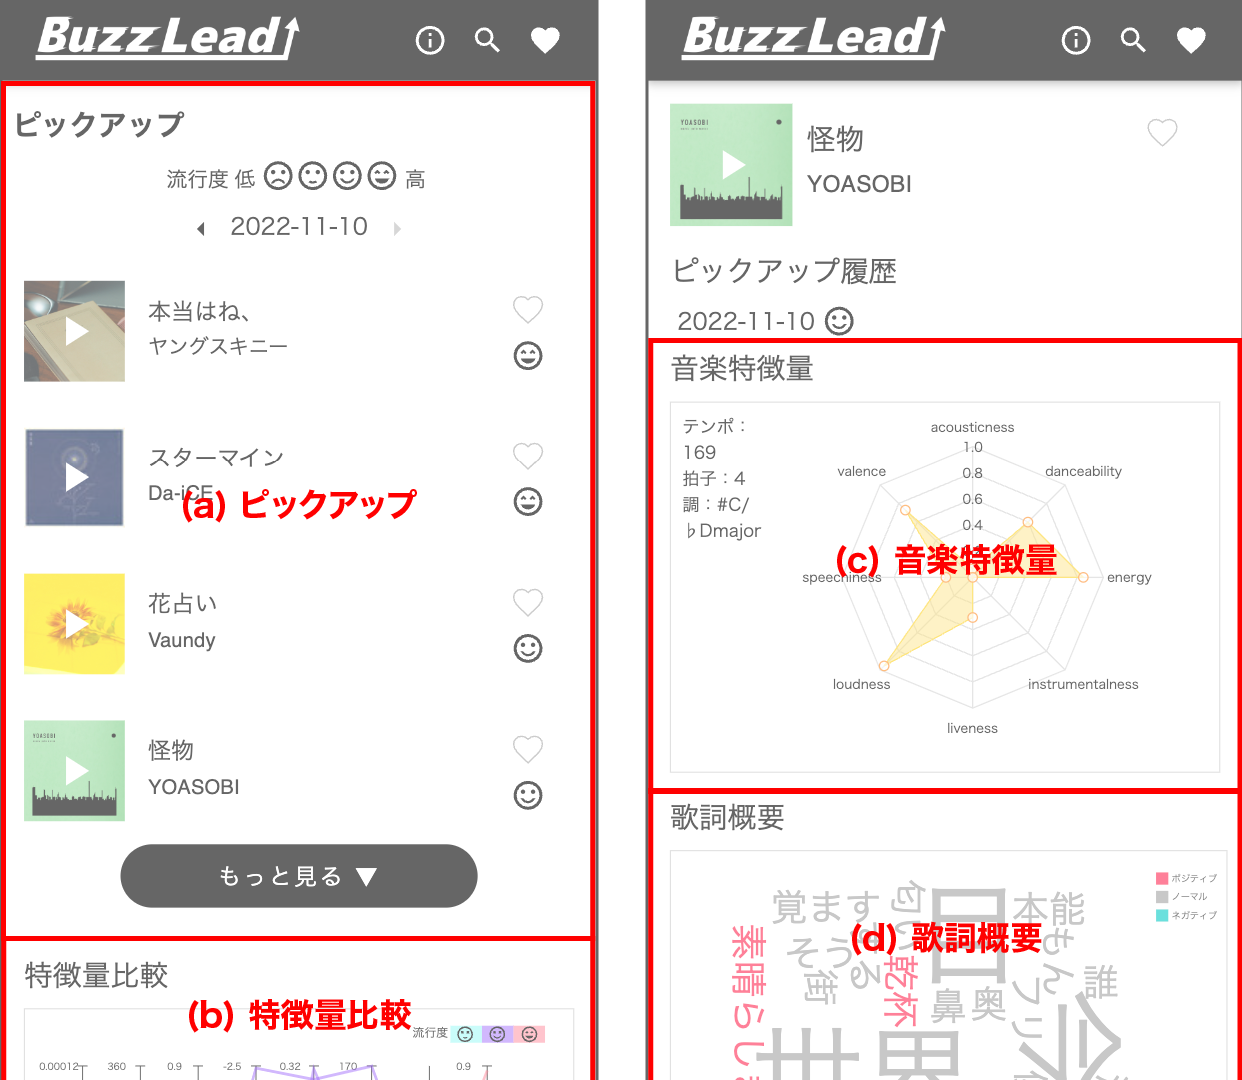
\includegraphics[width=120mm]{images/BuzzLead_sp.png}
\label{fig:smartphon}
\caption{
  TikTokの流行曲予測システムBuzzLeadのスマートフォンでのトップページと楽曲詳細ページのスクリーンショット.
  (a)ピックアップビュー:5.1と同様に選択した週に流行すると予測された楽曲を一覧表示する.
  (b)特徴量比較ビュー:5.1と同様にピックアップビューに表示されている楽曲の音楽特徴量を平行座標プロットによって表示する.
  (c)音楽特徴量ビュー:5.1と同様に選択された楽曲の音楽特徴量を表示する.
  (d)歌詞概要ビュー:5.1と同様に選択された楽曲の歌詞概要を表示する.
}
\end{center}
\end{figure}



\chapter{評価}
% R1~R4の要件を我々が開発したシステムが満たしているかは,hoge,hoge,hogeであることを確かめる必要があると考え,以下3項目を調査するために,予測の正確さの調査とユーザーテストを行った.
R1〜R4の要件を我々が開発したシステムが満たしているかどうかを確かめるために,以下の3項目の調査を行なった.
\begin{description}
\item [C1] 予測した楽曲が実際に流行したか
\item [C2] ユーザーが流行する楽曲の特徴を把握できたか
\item [C3] ユーザーが直感的にシステムを扱えたか
\end{description}


\section{予測の正確さ}
C1を明らかにするために,BuzzLeadでの流行曲の予測がどれくらい当たったかの割合を表\ref{table:predict_accuracy}に集計した.
TikTokで流行したかどうかはTikTok Chartsに楽曲名が載っているかどうかで判断している.
集計した結果の平均は12\%となった.
このような値になった原因として,まだ流行していない楽曲として集めた楽曲のデータにそもそもTikTokのランキングの曲が含まれていないことや,そもそもTikTok特有の楽曲などのSpotify Chartsにはない楽曲は取得できないことが考えられる.
前者に対しては,まだ流行していない楽曲として集める楽曲の幅を増やすことで解決できると考えている.
予測した楽曲が一切含まれていない週もいくつかあるが,9/29のように流行する楽曲を3割当てている週もある.
8/4の1曲,9/1の3曲,9/15の1曲,10/6の1曲,10/20の1曲はこれまでランキングに載っておらず,その週から流行し始めた楽曲をあらかじめ予測できていた.
%ユーザーに次流行する楽曲を提示するという目標を達成できたのではないだろうか.
また,これ以外の楽曲も,前の週に流行していた楽曲が次週も流行するのかどうかという点で,使用音源の流行を気にするユーザーが楽曲を選ぶ指標になると考えられる.
% だが,予測が当たる割合は低いので高めていきたい.
これらから,改善の余地はあるもののR1を満たすことができたと考えた.
\begin{table}[hbt]
% \begin{table*}[hbtp]
  \caption{予測の正確さ}
  \label{table:predict_accuracy}
  \centering
  % \begin{tabular}{ll}
  \begin{tabular}{c c c}
    \hline
    日付  & 割合  & 割合(\%)\\
    \hline \hline
    7/7 & 2/10 & 20\\
    7/14 & 2/12 & 17\\
    7/21 & 1/13 & 8\\
    7/28 & 0/9 & 0\\
    8/4 & 1/7 & 14\\
    8/11 & 0/9 & 0\\
    8/18 & 0/9 & 0 \\
    8/25 & 1/12 & 8\\
    9/1 & 3/15 & 20\\
    9/8 & 1/10 & 10\\
    9/15 & 2/9 & 22\\
    9/22 & 3/16 & 19\\
    9/29 & 2/6 & 33 \\
    10/6 & 1/11 & 9\\
    10/13 & 0/9 & 0\\
    10/20 & 1/11 & 9\\
    10/27 & 1/8 & 13\\
    % 11/3 & 1/4\\
    % 11/10 & /11\\
    \hline
  \end{tabular}
\end{table}

% \begin{table}[hbt]
% % \begin{table*}[hbtp]
%   \caption{予測の正確さ}
%   \label{table:predict_accuracy}
%   \centering
%   % \begin{tabular}{ll}
%   \begin{tabular}{c c c}
%     \hline
%     日付  & 割合  & 割合(\%)\\
%     \hline \hline
%     7/7 & 2/10 & 20\\
%     7/14 & 2/12 & 17\\
%     7/21 & 1/13 & 8\\
%     7/28 & 0/9 & 0\\
%     8/4 & 1/7 & 14\\
%     8/11 & 0/9 & 0\\
%     8/18 & 0/9 & 0 \\
%     8/25 & 1/12 & 8\\
%     9/1 & 3/15 & 20\\
%     9/8 & 1/10 & 10\\
%     9/15 & 2/9 & 22\\
%     9/22 & 3/16 & 19\\
%     9/29 & 2/6 & 33 \\
%     10/6 & 1/11 & 9\\
%     10/13 & 0/9 & 0\\
%     10/20 & 1/11 & 9\\
%     10/27 & 1/8 & 13\\
%     11/3 & 1/4 & 25\\
%     11/10 & 1/11 & 9\\
%     11/17 & 1/9 & 11 \\
%     11/24 & 1/14 & 7 \\
%     12/1 & 2/6 & 33 \\
%     12/8 & 0/13 & 0 \\
%     12/15 & 2/8 & 25 \\
%     12/22 & 3/11 & 27\\
%     12/29 & 2/11 &  18\\
%     1/5 & 0/25 & 0 \\ 
%     1/12 & 2/15 & 13\\
%     1/19 & 1/13 & 8\\
%     \hline
%   \end{tabular}
% \end{table}
    
\section{ユーザーテスト}
C2,C3を明らかにするためにユーザーテストを行った.
ユーザーテストに参加した実験参加者に,実際にBuzzLeadを操作してもらい,その後アンケートに回答してもらった.
% 最終的に33名の回答が得られた.
% ダンスや配信,音楽に関わっている団体にSNSで拡散をした.実際にBuzzLeadを使用してもらい,アンケートを行った結果,33名の回答が得られた.
\subsection{実験参加者}
実験参加者は,情報科学を専攻する大学生13名と,ダンスや配信,音楽に関わっている団体への募集で集まった20名の33名である.
33名のうち,TikTokを普段利用する人は13名,その中でも配信をする人は3名だった.
また,TikTok以外のツールで動画の配信を行っている人は6名だった.
%88\%が20~25歳,その他は10代と25~29歳だった.また,

\subsection{アンケート結果}
BuzzLeadで表示しているピックアップ曲や,楽曲詳細などのビューについての評価をするために,5段階評価(5:そう思う,4:ややそう思う,3:どちらともいえない,2:あまりそう思わない,1:全くそう思わない)で次のQ1〜Q5の質問を行った.
\begin{description}
\item [Q1] 選択した楽曲の音楽の特徴を知ることができた
\item [Q2] 選択した楽曲の歌詞の特徴を知ることができた
\item [Q3] 選択した楽曲の歌詞がどれくらいポジティブかを知ることができた
\item [Q4] 選択した楽曲の歌詞がどれくらい韻を踏んでいるかを知ることができた
\item [Q5] 自分の検索した楽曲の流行度を知ることができた
\end{description}
Q1〜Q5の結果(図2)から多くの実験参加者が楽曲詳細のビューを用いて音楽,歌詞両方の特徴を掴むことができていることがわかる.
これより,R2,3を満たしていると考えられる.
% 一方Q6では票がバラけており,お気に入りに登録した曲の共通点を見つけることが少し難しかったと考えられる.
% これは,ピックアップの下にある特徴量比較のようなビューをマイページに設けていなかったことが原因と考えられるため,そのような複数曲を比較できるビューをマイページにも設けるようにしていきたい.

システムの操作が関わるQ1〜Q5に加え,楽曲検索を行えたかどうか,マイページにお気に入りを登録することができたかどうかといった質問では,30名以上が4か5を選択しており,実験参加者が直感的にシステムを扱うことができていたと考えられる.

一方,実験参加者に対して「ピックアップ」に表示されているのはどのような楽曲か聞いたところ,今,TikTokで流行っている楽曲と回答した人が42\%,正解であるこれからTikTokで流行しそうな楽曲と回答した人が27\%,その他が31\%とこちらの意図が伝わっていない結果となった.
この結果から,このアプリケーションの目的が実験参加者にしっかり伝わっていなかったことと,流行度という言葉を既に流行しているものを表していると認知した実験参加者が一定数いたためだと考えられる.
流行度やピックアップという題名を考え直すと共にUIの改善を行っていきたい.

以上のことから,一部UIに改善点はあるもののR4を達成することができたと考える.
\begin{figure}[htb]
\begin{center}
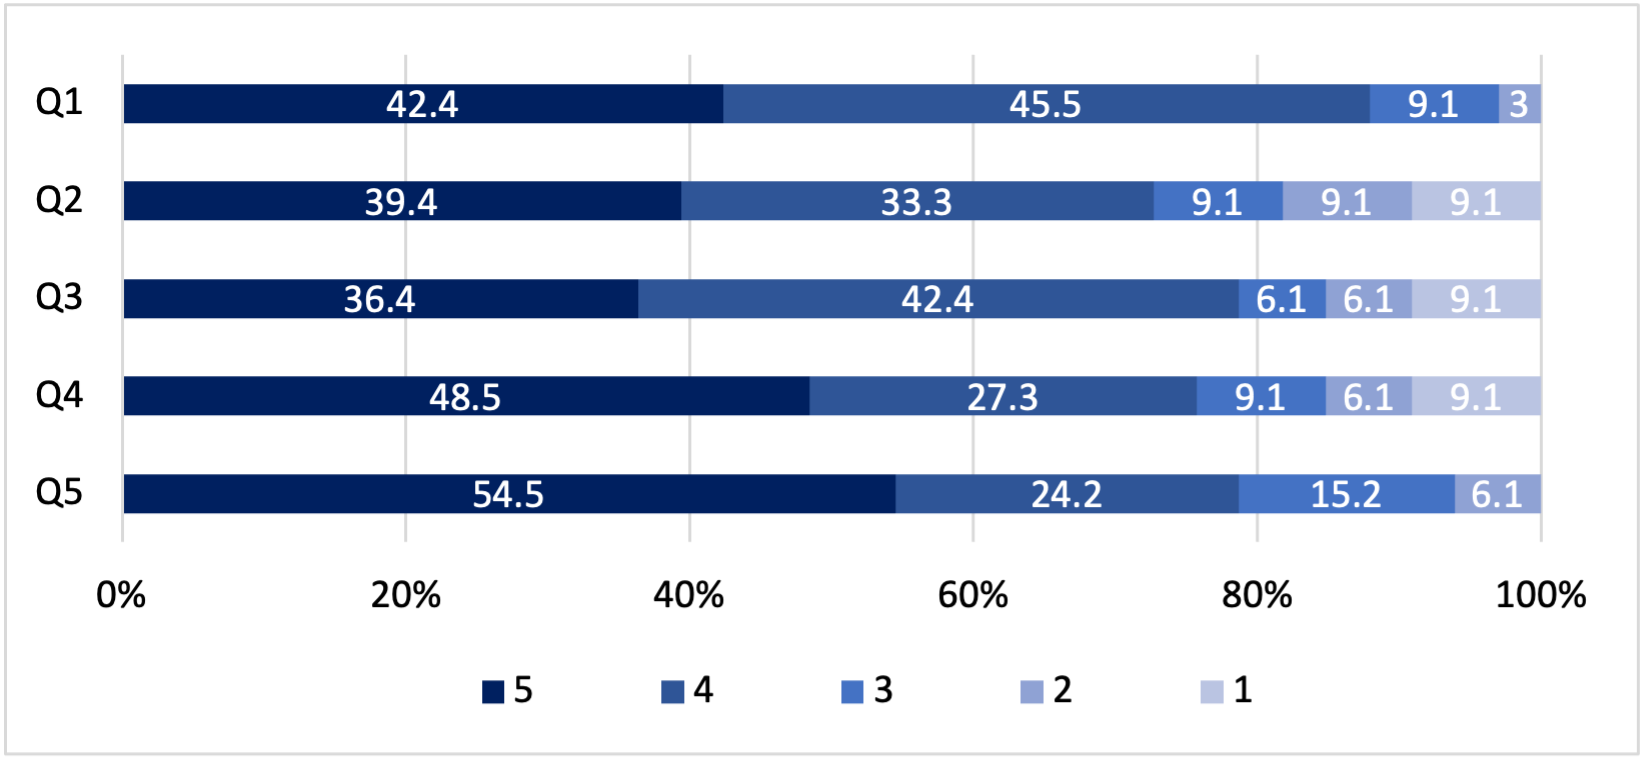
\includegraphics[width=80mm]{images/feature.png}
\label{table:detail}
\caption{楽曲詳細}
\end{center}
\end{figure}

%前向きな意見
%古い曲を調べると流行度が低いことが多かったので,ある意味正確なように感じました.ただ,今実際にtiktokで流行しているものを知らないので本当に流行するのかどうかはわからないと思いました.
%可視化についても流行度を色で,音楽の特徴量を折れ線で表現することで1つのチャートで表せていたりしていて直感的に理解できるように感じました.
%流行っていた曲の特徴を知ることができたので,これから流行する曲がどのような曲調のものなのかを少し予想できるようになりました.

%改善点
%ピックアップ履歴というところに流行度の推移が表示されており,これが何かわからなかった.
%音楽に対して詳しくないので音楽の特徴を見ても,何が理由で流行しそうなのかわからなかった.
%自分が見たのが悪かったのがdanceability,energy,loudnessが大体同じくらい高いしspeechiness,instrumentalnessは大体0で差を感じなかった.
%歌詞のポジティブとネガティブ,曲の韻踏み度とポジティブ度,それらが流行しそう度とどう関係があるのかわからない←未実装の伝達不足
%曲同士の比較がもっとできると嬉しい
%月や年単位でのピックアップorランキングの表示
%その他UIの改善


%\subsection{サービス全体について}
最後にサービス全体についても5段階評価でQ6〜Q8の質問を行った.
\begin{description}
\item [Q6] 流行しそうな楽曲を知ることができた
\item [Q7] 流行しそうな楽曲の特徴を掴むことができた
\item [Q8] 実際におすすめされた楽曲を使って動画を投稿してみようと思った
% \item [Q10] オススメされた流行度の高い楽曲が実際に流行しそうだと思った
\end{description}
その結果を図3に表す.
Q6,Q7に関しては前向きな評価を多く得ることができ,R1,R2を達成できたと考えることができる.
% また,Q10でも多くの人が5か4を回答していることから提示した曲が直感的にも流行しそう
一方,Q8では5,4をつけた人が少なかった.
今回の実験参加者に,TikTokで動画投稿をしている人が3名しかいないからだと考えられる.
TikTok投稿を行なっている人の評価は4,3,1であった.
% これは5.2.1にもあるように,今回の参加者に,そもそもTikTokで動画投稿をしている人が少ないからだと考えたが実際はそうでもなかった.Q9で4,5の評価をしてくれた人は,動画投稿をする人が2名,しない人が3名だった. また,実際にTikTok投稿を行なっている人の評価は4,3,1であった.

\begin{figure}[htb]
\begin{center}
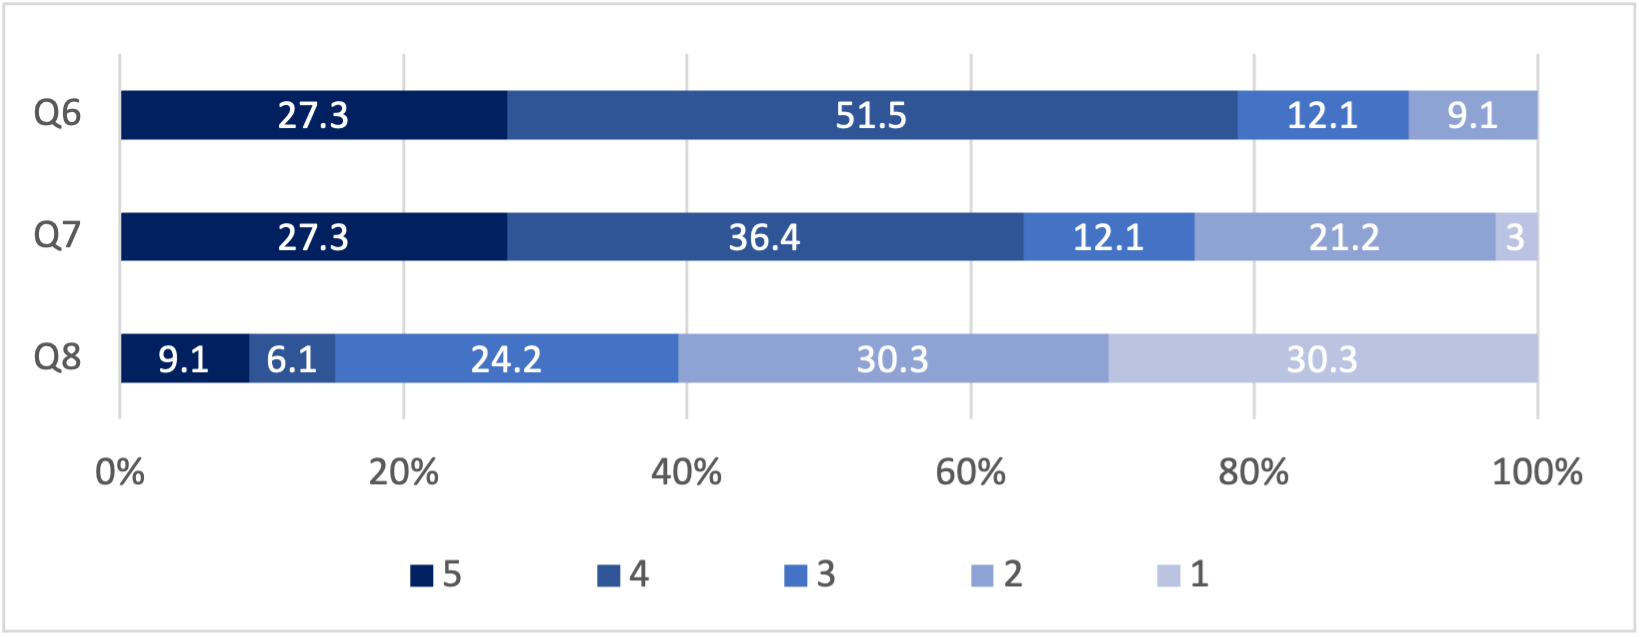
\includegraphics[width=80mm]{images/all.png}
\label{table:total}
\caption{サービス全体について}
\end{center}
\end{figure}

以下は,実験参加者の自由記述によるコメントの抜粋である.
\begin{itemize}
\item 古い曲を調べると流行度が低いことが多かったので,ある意味正確なように感じました
\item 流行っていた曲の特徴を知ることができたので,これから流行する曲がどのような曲調のものなのかを少し予想できるようになりました.
\item 歌詞のポジティブとネガティブ,曲の韻踏み度とポジティブ度,それらが流行しそう度とどう関係があるのかわからない
\item 月や年単位でのピックアップorランキングの表示
\end{itemize}
コメントから,実験参加者は流行度に納得していることや流行する楽曲の特徴を掴めていることがわかる.
一方で,歌詞特徴量が流行度とどう関係しているかわからないという意見もあった.
これは,流行度の算出に歌詞特徴量を使用していないことや,特徴量比較ビューに歌詞特徴量を表示していないためだと考えられる. 
現時点で,歌詞取得が楽曲の冒頭部分しかできていないため音楽特徴量のみを使用しているが,全歌詞を使用した歌詞特徴量の採用は今後の課題である.
最後に,月や年単位でのピックアップあるいはランキングの表示をしてもらいたいとの意見もあったので検討していきたい.


\chapter{考察}
本研究ではTikTokでこれから流行する楽曲や,ユーザーの使用したい楽曲が流行するかどうかを提示するシステムの開発を目標に掲げ,4つのシステム要件を定めた.

R1に関しては,6.1にもあるように一部予測はできているが精度が低い結果となった.
しかし, TikTok Chartsの順位が大きく入れ替わる際に予測した楽曲がランクインしていることもあり,精度は低いながらも要点はつかめている印象を受けた.
今回はこのような精度となったが,歌詞を利用した分類や,楽曲全体ではなくサビやAメロといった楽曲の一部分を対象にした分類を行うと,よりTikTokの傾向に沿った予測ができるのではないかと考えている.

R2に関しては,6.2.2にあるように多くのユーザーが楽曲の特徴を把握できていた.
しかし歌詞が冒頭しか取得できていないことから,楽曲全体の歌詞の特徴を掴むのには適していない状態となってしまった. 
歌詞の取得先を変更するなどの改善を行っていきたい.

R3に関しては,ユーザーが検索した楽曲の流行度をアイコンで提示することで達成できた.
また,流行度の高い類似曲を提示することでユーザーの嗜好に合致し,かつ流行しやすい曲を把握することが可能になった.

R4に関しては,タイトルの付け方によってユーザーの誤解を招いてしまう部分があったが,多くのユーザーが問題なくアプリケーションを操作していた. 
また,スマートフォンを利用してユーザーアンケートに回答したユーザーは45\%を占めていた.この結果から,レスポンシブデザインを取り入れたことにより,TikTokを使用しているユーザーのアンケート協力の件数を増やすことができたと感じている.

全体を通して,予測の精度は改善の余地があるがアプリケーションとしては要件を満たすものが作成できた.
TikTokで自身のコンテンツを流行させたい人はもちろんだが,著者の一人も一時期TikTokの投稿をする際に使用楽曲を選ぶ煩わしさを感じていたので,そういった人達の助けにもなることを願っている.

% 実際やる前から曲の共通点出すの難しくね?ってなってて、わかったらやばいねって話を音楽友達としてたり。で、実際学習させてみてもまぁそうよねって感じではあったので、そうだよなって感じではある。世の中ほんと色んな楽曲があって、これが一番流行る!とかは一概に言えないんだなって再認知したというかなんというか。
% そんな中でも、大バズりしてる楽曲は流行度が高いことが多くて、なんらかはあるんだろうなと思ったり、でもぱっと見わからない。誤差なんか。
% TikTok一回バズるとだいたいその曲が数週間ずっとランキング上位にいるんだけど、それがひっくり返るタイミングで予想曲当ててたのはちょっと胸熱だった。
% 歌詞を利用しての分類や, 楽曲全体ではなくサビやAメロといった一部分のみでの分類等を行うとまた違った結果になるのではないかと思っている。TikTokは15秒とかしか使わないから、そこだけで見てみたいっていうやつ。
% ユーザーインターフェースというかアプリケーションとしての機能はそれなりにできていたと思う。レスポンシブデザインも用意して、実際にテストでスマートフォンを使うユーザーもいて狙い通りだった。一部文言での伝達ミス?があったりレイアウトや、楽曲再生などまだ改善点はあるけどそれっぽいものはできたのでは。
% TikTok投稿は2年前とかに一時期広報で使ってて曲選ぶのはめんどかったから、そういう人の助けになったらいいなと思ったり

\chapter{おわりに}
本研究では,TikTokで流行っている楽曲のデータを用い,楽曲選定の支援を目的としたシステムであるBuzzLeadを開発した.
音楽特徴量を用いてどのような特徴を持つ楽曲が流行するのか,自身の選んだ楽曲は流行しそうなのかを予測・提示することができた.
評価実験によって,ピックアップとしてシステムが提示した楽曲が実際に次の週のTikTok Chartsに掲載されていることが確認できた.
以上から我々の目的を達成できるシステムを開発することができたと考えられる.

一方で,改善点として挙げられるのがユーザーに目的を伝えきることができなかった「ピックアップ」という項目である.
TikTokで流行った楽曲の情報をもとに今後流行するであろう楽曲を提示するのが目的であったが,今現在TikTokで流行っている楽曲であると認識しているユーザーが42\%を占めた. 
回答の中にはSpotifyに関する項目であるというものも散見され,ここで目的が伝わりきらなかった理由について「このアプリケーションがどのようなものか理解せずにユーザーが利用している」ということが原因として考えられる.
どのような目的を持って作られたアプリケーションであるのかという文言をウォークスルーに盛り込むなどして改善を行っていきたい. 

\chapter*{謝辞}
% 先生ありがとうーーーーー
本研究を遂行するにあたり,指導教官である日本大学文理学部情報科学科尾上准教授には終始多大なご指導をいただきました.心から感謝いたします.
また,本研究の遂行にあたり,快く実験に参加頂いた皆様に感謝いたします.
% さんまのっけて大丈夫?
最後に,本研究を半年間協力して頂いた伊藤和斗氏,松永大氏をはじめ,尾上研究室の皆様には,本研究の遂行にあたり多大なご助言,ご協力を頂きました.本当にありがとうございました.

\begin{thebibliography}{10}
% \bibitem{paper0}
% 池上 真平,佐藤 典子,羽藤 律,生駒 忍,宮澤 史穂,小西 潤子,星野 悦子:
% 日本人における音楽聴取の心理的機能と個人差,
% 心理学研究,VOL.92,No.4,p.237-247(2021).

\bibitem{paper1}
矢倉 大夢,中野 倫靖,後藤 真孝: 
作業用BGMに特化した楽曲推薦システム,
情報処理学会研究報告,Vol.2016-MUS-112,No.3(2016).

\bibitem{paper2}
佐久間廉,伊藤 克亘: 
投稿データを利用した動画投稿者のためのBGM推薦システム,
第84回全国大会講演論文集,VOL.2022,NO.1,p257-258.

\bibitem{paper10}
小野佑大,石先広海,帆足啓一郎,小野智弘,甲藤二郎:
音楽のムード分類結果を利用したホームビデオへのBGM付与支援システム,
情報科学技術フォーラム講演論文集,VOL.9,No.2,p295-296(2010年)

\bibitem{paper4}
韓語佳,中野美由紀,小口正人:
利用者の印象に基づく高齢者向け音楽推薦システム「元気フクロウ」-嗜好に合わせた適応的推薦手法の提案-,
第84回全国大会講演論文集,VOL.2022,NO.1,p535-536.

\bibitem{paper5}
馬場南斗,岡田龍太郎,峰松彩子,中西崇文:
楽曲メディアコンテンツを対象とした動画メディアコンテンツの色彩特徴に起因する印象に合致した楽曲推薦システムの構築,
第84回全国大会講演論文集,VOL.2022,NO.1,p531-532.

\bibitem{paper9}
小林 恭輔,高久 雅生:
楽曲探索を支援するための類似楽曲提示手法,
VOL.32,NO.2,p287-293(2022).

\bibitem{paper6}
神野満里奈,福原義久:
歌詞や曲調の印象に応じた舞台照明の自動調光・調色システムの実現,
第83回全国大会講演論文集,VOL.2021,NO.1,p743-744.

\bibitem{paper3}
鍵田 里沙子,山西 良典,西原 陽子,福本 淳一:
表現特徴に着目した歌詞の印象的フレーズ抽出,
情報処理学会研究報告,VOL.2013-MUS-101,NO.6(2013).


\bibitem{paper7}
CAO CHONG:
日本語曲を原曲とする中国語カバー曲における歌詞の押韻率と意味合致度の分析, 
筑波大学修士(情報学)学位論文(2017).


\end{thebibliography}



\end{document}

aper5}
馬場南斗,岡田龍太郎,峰松彩子,中西崇文:
楽曲メディアコンテンツを対象とした動画メディアコンテンツの色彩特徴に起因する印象に合致した楽曲推薦システムの構築,
第84回全国大会講演論文集,VOL.2022,NO.1,p531-532.

\bibitem{paper9}
小林 恭輔,高久 雅生:
楽曲探索を支援するための類似楽曲提示手法,
VOL.32,NO.2,p287-293(2022).

\bibitem{paper6}
神野満里奈,福原義久:
歌詞や曲調の印象に応じた舞台照明の自動調光・調色システムの実現,
第83回全国大会講演論文集,VOL.2021,NO.1,p743-744.

\bibitem{paper3}
鍵田 里沙子,山西 良典,西原 陽子,福本 淳一:
表現特徴に着目した歌詞の印象的フレーズ抽出,
情報処理学会研究報告,VOL.2013-MUS-101,NO.6(2013).


\bibitem{paper7}
CAO CHONG:
日本語曲を原曲とする中国語カバー曲における歌詞の押韻率と意味合致度の分析, 
筑波大学修士(情報学)学位論文(2017).


\end{thebibliography}



\end{document}

